% !TeX spellcheck = en_US
% !TeX encoding = UTF-8
% !TEX program = pdflatex

% VSCODE word wrap: ALT + Z
% COMPILE WITH:
% `latexmk` 
% latexmk -pdf main.tex
% You need pdflatex and biber (in all TeXLive distributions)

\documentclass[11pt]{article} % text width
\usepackage[utf8]{inputenc} % encode text to utf8


% paragraph formatting: https://www.overleaf.com/learn/latex/Paragraph_formatting
\setlength{\parindent}{1em}
\setlength{\parskip}{1em}


% better language support
\usepackage[english]{babel}

% use pdflatex
\usepackage[T1]{fontenc} % font encoding
\usepackage[a4paper, margin=2cm, head=18.0pt]{geometry} % set margins to 1.5 cm
\usepackage{graphicx}% for graphics
\usepackage{float}
\usepackage[onehalfspacing]{setspace}
\usepackage{tocbasic}
\usepackage{booktabs}
\usepackage{multicol}
\usepackage{multirow}
\usepackage[]{scrlayer-scrpage}
\usepackage[titletoc]{appendix}
\usepackage{comment}
\usepackage{csquotes}% quote

% quotes and bibliography: https://www.overleaf.com/learn/latex/Typesetting_quotations
\usepackage{csquotes}
\usepackage{dirtytalk}
\DeclareQuoteStyle{english}{\glqq}{\grqq}{\glq}{\grq}

% \usepackage[
%     backend=biber,
%     style=numeric,
%     sorting=none
% ]{biblatex}
\usepackage[backend=biber, style=numeric, defernumbers=true]{biblatex}
% add commands for automatic cite/uncite distinction
\DeclareBibliographyCategory{cited}
\AtEveryCitekey{\addtocategory{cited}{\thefield{entrykey}}}
\addbibresource{biblio.bib} % bibliography
\nocite{*} % all references

\newcommand{\ts}{\textsuperscript} % superscript for 2nd or XIXème

\pagenumbering{roman} % set page numbering of front matter sections

% use acronyms and glossaries
% toc: add glossary to table of contents
\usepackage{hyperref}
\usepackage[acronym, toc]{glossaries} 
\makeglossaries
% technical terms
\newacronym{vmi}{VMI}{Virtual Machine Introspection}
\newacronym{ssh}{SSH}{Secure Shell}
\newacronym{regex}{REGEX}{regular expressions}
\newacronym{scp}{SCP}{secure copy}
%static analyse
\newacronym{bfd}{BFD}{Byte Frequency Distribution}
%deep learning
\newacronym{lstm}{LSTM}{Long Short-Term Memory}
\newacronym{gru}{GRU}{Gated Recurrent Units}
\newacronym{rnn}{RNN}{Recurrent Neural Networks}
\newacronym{cnn}{CNN}{Convolutional Neural Networks}
\newacronym{rcnn}{RCNN}{Recurrent Convolutional Neural Network}

\newacronym{seq2seq}{Seq2Seq}{Sequence-to-Sequence}
% machine learning
\newacronym{smote}{SMOTE}{Synthetic Minority Over-sampling Technique}
\newacronym{pca}{PCA}{Principal Component Analysis}
\newacronym{t-sne}{t-SNE}{t-Distributed Stochastic Neighbor Embedding}

\newacronym{knn}{KNN}{K-Nearest Neighbors}
\newacronym{svm}{SVM}{Support Vector Machines}



% glossaries
\newglossaryentry{pointer}
{
    name=pointer,
    description={In our study, pointers are characterized as sequences of hexadecimal numbers that reference distinct memory addresses. These sequences can be recognized using the following regular expression: \texttt{"[0-9a-f]{12}0{4}"}}
}

\newglossaryentry{structure}
{
    name=structure,
    description={In our study, structures are defined as a series of bytes that are allocated in the heap. These structures are allocated using the \texttt{calloc} function and begin everytime by a \textit{malloc header}}
}


\begin{comment}
\newglossaryentry{nodes}
{
    name=nodes,
    description={A node is an entity in a graph, it can be a person, a place, a thing, or any other entity.}
}

\newacronym{kg}{KG}{Knownledge Graph}
\newacronym{foss}{FOSS}{Free and Open Source Software}
\newacronym{rdf}{RDF}{Resource Description Framework}
\newacronym{rdfs}{RDFS}{Resource Description Framework Schema}
\newacronym{owl}{OWL}{Web Ontology Language}
\newacronym{ml}{ML}{Machine Learning}
\newacronym{nlp}{NLP}{Natural Language Processing}
\newacronym{ke}{KE}{Knowledge Engineering}
\newacronym{del}{DEL}{Directed Edge-labelled Graphs}
\newacronym{er}{ER}{Entity Resolution}
\newacronym{qa}{QA}{Quality Assurance}
\newacronym{sparql}{SPARQL}{SPARQL Protocol and RDF Query Language}
\newacronym{gnn}{GNN}{Graph Neural Network}
\newacronym{gcn}{GCN}{Graph Convolutional Networks}
%\input{glossaries.tex} % acronyms definitions, failed to make in work on a separate file!!!
\end{comment}

% custom commands
% escape char in latex: https://tex.stackexchange.com/questions/34580/escape-character-in-latex
% horizontal spacing: https://tex.stackexchange.com/questions/74353/what-commands-are-there-for-horizontal-spacing/74354
\newcommand{\p}{\texttt{+}} % small unary plus
\newcommand{\doublep}{\texttt{++}} % double small unary plus
\newcommand{\m}{\texttt{-} \space} % small unary minus
\newcommand{\doublem}{\texttt{-}\texttt{-} \space} % double small unary minus

% code 
\usepackage{listings}
\usepackage{hyphenat} % fix "overfull hbox" with slicing words using hyphenation
\hyphenation{hy-phen-a-tion} % indicate all 3 permissible hyphenation points

% where to put all images and figures
\graphicspath{{img/}}

% customize the header and footer of the document
\usepackage{scrlayer-scrpage}
\clearpairofpagestyles
\cfoot[\pagemark]{\pagemark}

% document info
\newcommand{\thetitle}{Structure embeddings for OpenSSH heap dump analysis}
\newcommand{\theauthor}{Lahoche, Clément Claude Martial}

\title{\thetitle}
\author{\theauthor}
\date{\today}

% document content
\begin{document}

% !TeX spellcheck = en_US
% !TeX encoding = UTF-8
\begin{titlepage}
    \centering
    \begin{onehalfspace}
    	
		
\includegraphics[width=7cm, height=1.5cm]{uni-logo.png}
		\hspace*{1.0cm}
		\includegraphics*[width=7cm, height=1.5cm]{Logo_INSA.png}\\
		\vspace{1.0cm}
        	{\Large \bfseries Masterarbeits }\\

        	\vspace{2.5cm}

            \begin{doublespace}
            	{\textsf{\Huge{\thetitle}}}
            \end{doublespace}

        	\vspace{2cm}

            {\Large A report by}\\

        	\vspace{1cm}

        	{\bfseries \large{\theauthor} }\\ ORCID id : 0009-0007-7687-5419
			

        	\vfill

        	{\Large
                \textsc{Pr\"ufer} \\
				Prof. Dr. Harald Kosch \\
                Prof. Dr. Michael Granitzer\\
        	}

        	\vspace{1.5cm}

        	\parbox{\linewidth}{\hrule\strut}

            \vfill

			{\large \today}
    \end{onehalfspace}
\end{titlepage}

\newpage

%%%%%%%%%%%%%%%%%%%%%%%%%%%%%%%%%%%%%%%%%%%%%%%%%%%%%%%%%%%%%%%%%%%%%%%%%%%%%%%%%%%%%%%%%

% -- ABSTRACT
\section*{Abstract}

% -- Acknowledgements
\section*{Acknowledgements}


\newpage

% table of content with list of figures & tables
\tableofcontents
\listoffigures
\listoftables
\newpage

%%%%%%%%%%%%%%%%%%%%%%%%%%%%%%%%%%%%%%%%%%%%%%%%%%%%%%%%%%%%%%%%%%%%%%%%%%%%%%%%%%%%%%%%%
\pagenumbering{arabic} % reset page numbering of main matter sections
\begin{comment}
\section{Introduction and History}

\subsection{Motivation}
Knowledge Graphs are now widely used in many applications, such as search engines, virtual assistants, and social media platforms. Their usage span over many domains ranging from drug discovery to fraud detection passing by smart manufacturing. The current report is based mainly on \citetitle*{KG21} and similarly tries to introduce the subject of Knowledge Graphs to the seminar participants. It discusses what are Knowledge Graphs, the history behind, and introduces related concepts like \acrshort{kg} construction, or reasoning techniques. The oral presentation has been given on the 7th of June 2023, under the supervision of Prof. Dr. Alsayed Algergawy, with Andreas Einwiller as monitor. This presentation was the first one of the seminar and was followed by a discussion session. The current report is based on the presentation and the discussion session.

\subsection{Historical Evolution of Knowledge Engineering (KE)}
The history and evolution of the knowledge engineering discipline has seen significant transformation since its inception during the expert systems development phase in the 1980s. Four different periods can be distinguished, ranging from 1955 to the present day, with each period introducing new requirements for knowledge production processes to overcome the limitations of systems developed in preceding periods \cite*{KGKE22}.

\begin{itemize}
    \item \textbf{Dawn of AI:} The initial focus was on reliable and effective processes.
    \item \textbf{Expert Systems Era:} Feigenbaum stressed the need for domain-specific focus for automated knowledge production, leading to the creation of expert systems. However, these systems proved to be brittle and hard to maintain, thus the need for scalable, globally distributed, and interoperable systems arose.
    \item \textbf{Semantic Web Era:} Tim Berners-Lee advocated for a “Web of Data” based on linked data principles, standard ontologies, and data sharing protocols. This period saw the development of a globally federated open linked data cloud and techniques for ontology engineering. However, wider adoption was slow and led to the call for more developer-friendly tools and methods to deal with data noise and incompleteness.
    \item \textbf{Language Model Era:} Language Learning Models or Large Language Models (LLMs) are now ubiquitous due to recent advancements in neural network architectures and graphical processing hardware. Language models can either serve as knowledge bases that are queryable using natural language prompts or as a component in a knowledge production workflow.
\end{itemize}

All thoses differents phases have seen the development of new concepts, tools and methods to deal the ever growing complexity of the knowledge production processes and analysis. In the wake of Google's announcements in 2012 \cite*{googleblog2023knowledgegraph}, the last decade has seen the development of Knowledge Graphs as a powerful approach to organizing and structuring real-world information by modeling entities, their properties, and the relationships between them. 

\section{What is a Knowledge Graph?}

\subsection{Knowledge and Graph Theory}
Defining knowledge is not a straightforward task, so this report will focus on "explicit knowledge". Explicit knowledge is defined as "something that is known and can be written down" \cite[p.4]{KG21}. It is composed of statements, such as sentences, that draw relationships between concepts and data.

Graph theory is a field that lies at the intersection of computer science and mathematics and is concerned with the study of graphs. A graph is a type of data structure consisting of nodes (also known as vertices) and edges (or arcs) that connect pairs of nodes. Graph theory is used to model and analyze various types of relationships and structures in a wide range of fields, including computer networks, social networks, biological networks, and many others.

A Knowledge Graph can be defined as \say{a graph of data intended to accumulate and convey knowledge of the real world, whose nodes represent entities of interest and whose edges represent potentially different relations between these entities} \cite[p.3]{KG21}. \say{Knowledge graphs serve as a common substrate of knowledge within an organization or community, enabling the representation, accumulation, curation, and dissemination of knowledge over time} \cite[p.31]{KG21}.

\subsection{Knowledge Graphs}
\say{At the foundation of any knowledge graph is the principle of first modelling data as a graph} \cite[p.4]{KG21}. A Knowledge Graph is thus a data graph intended to accumulate and convey real-world knowledge. The nodes in the graph represent entities, and the edges represent relations between these entities. It serves as a common substrate for knowledge representation that is both flexible and extendable.

\subsubsection*{A difficult definition}
The term "knowledge graph" first appeared in 1973, but really gained popularity through a 2012 blog post about Google's Knowledge Graph \cite*{googleblog2023knowledgegraph}. According to litterature, below are listed some of the most common definitions of Knowledge Graphs:
\begin{itemize}
    \item \say{A knowledge graph acquires and integrates information into an ontology and applies a reasoner to derive new knowledge.} \cite{TDKG16}
    \item \say{A graph of data intended to accumulate and convey knowledge of the real world, whose nodes represent entities of interest and whose edges represent potentially different relations between these entities.} \cite{KG21}
    \item \say{A graph of data consisting of semantically described entities and relations of different types that are integrated from different sources. Entities have a unique identifier. KG entities and relations are semantically described using an ontology or, more clearly, an ontological representation.} \cite{CKG23}
\end{itemize}

The very nature of KG makes any definition attempt difficult. Indeed, KG is a broad concept that can be applied to many different domains, use cases and can have diverse implementations. The definition of KGs is thus very context-dependent. However, the common denominator of all KGs is that they are graphs of data that represent some knowledge or information in a graph-structured representation.

\subsubsection*{Understanding KG}

Graphs offer a flexible way to conceptualize, represent, and integrate diverse and incomplete data. \say{Knowledge graphs use a graph-based data model to capture knowledge in application scenarios that involve integrating, managing and extracting value from diverse sources of data at large scale} \cite[p.2]{KG21}. They have a number of benefits when compared with a relational model or NoSQL alternatives, such as the ability for data to evolve in a more flexible manner, and the capacity to organize data in a way that is not hierarchical. They can represent incomplete information, and does not require a precise schema \cite[p.2]{KG21}.

\subsubsection*{Types of KG}
Knowledge graphs can adopt any graph data model, and data can typically be converted from one model to another. Some of the different types of graphs include:

\begin{itemize}
    \item \textbf{Directed Edge-labelled Graphs (DEL):} The classic graph, set of nodes and edges that connect the nodes with in certain way. \acrshort{rdf} is a popular \acrshort{del} data model.
    \item \textbf{Heterogeneous Graphs:} Each node and edge is assigned one type, allowing for partitioning nodes according to their type, which is useful for machine learning.
    \item \textbf{Property Graphs:} Allows a set of property-value pairs and a label to be associated with nodes and edges. This model is used in Neo4j and offers great flexibility but is harder to handle and query.
    \item \textbf{Graph Dataset:} A set of named graphs, with a default graph with no ID. Useful when working with different sources.
    \item \textbf{Hypergraphs:} Allow edges that connect sets rather than pairs of nodes.
\end{itemize}


\subsection{Applications and Use Cases}

Knowledge Graphs have found widespread application in both open source, research and enterprise contexts. Open Knowledge Graphs are publicly accessible and often integrate data from various sources, while enterprise Knowledge Graphs are typically proprietary and used internally within organizations.

\subsubsection*{Open Knowledge Graphs}

Several Open Knowledge Graphs have been developed, including:

\begin{itemize}
    \item \textbf{BabelNet:} Integrates several resources including Wikipedia and WordNet to provide multilingual lexical knowledge.
    \item \textbf{DBpedia:} Extracts structured content from Wikipedia to make it accessible on the Web.
    \item \textbf{Freebase:} A crowdsourced database of well-known people, places, and things.
    \item \textbf{Wikidata:} Serves as the central storage for the structured data of Wikimedia projects.
    \item \textbf{YAGO:} Automatically extracts and integrates knowledge from Wikipedia and other sources.
\end{itemize}

\subsubsection*{Enterprise Knowledge Graphs}

Enterprise Knowledge Graphs are used in various industries including web search, commerce, social networks, and finance. Some examples include:

\begin{itemize}
    \item \textbf{Google Knowledge Graph:} Enhances Google Search's results with semantic-search information gathered from various sources.
    \item \textbf{Amazon Product Knowledge Graph (PKG):} A large-scale, semi-structured knowledge graph that organizes information about products sold on Amazon and relationships between them.
\end{itemize}

These Knowledge Graphs are used in a wide range of applications including search, recommendations, information extraction, personal agents, advertising, business analytics, risk assessment, automation, and more.

\section{Advanced Topics in Knowledge Graphs}

\subsection{Construction, Creation, Extraction}

Building Knowledge Graphs often require physical data integration systems that amalgamate information from a variety of sources into a logically centralized, graph-like representation. This creation process often involves integrating data from diverse sources, including direct human input, extraction from existing text, markup, legacy file formats, csv or json files, relational databases, or even other knowledge graphs. 

The construction of KGs involves several tasks. The initial step often consists in data acquisition and preprocessing. This phase involves the selection of relevant sources, acquisition and transformation of relevant source data, as well as initial data cleaning. Since the data used can be of diverse types, metadata management is important so as to deal with different kinds of metadata like the provenance of entities, structural metadata, temporal information, quality reports, and process logs. The complexity of integrating diverse data from different sources also lies in the ontology management. A simple approach to this is to allow incremental evolution of the ontology, but this can lead to inconsistencies and incoherences.

Once the KG is in place, more valuable information can be extracted from it: this is the knowledge extraction phase. Knowledge Extraction (\acrshort{ke}) refers to the derivation of structured information and knowledge from unstructured or semi-structured data. This can be done through a range of techniques such as entity resolution and fusion, quality assurance, and knowledge completion. Entity Resolution (\acrshort{er}) and Fusion involves the identification of matching entities and their fusion within the KG. Quality Assurance (\acrshort{qa}) involves identifying and repairing data quality problems in the KG. Knowledge Completion involves extending a given KG, for example, by learning missing type information, predicting new relations, and enhancing domain-specific data.

\subsection{Search and Querying}

Querying KGs often involves the use of graph query languages such as \acrshort{sparql} for \acrshort{rdf} graphs and Cypher, Gremlin, and G-CORE \cite{KG21} for property graphs. These languages allow for the creation of graph patterns, which are graphs similar to the data being queried that can contain variables so that they can be evaluated to retrieve information from constants in the KG. Graph patterns can follow either homomorphism-based semantics, which allow multiple variables to be mapped to the same term, or isomorphism-based semantics, which require variables on nodes and/or edges to be mapped to unique terms.

In more complex scenarios, Complex Graph Patterns and Navigational Graph Patterns can be used. Complex Graph Patterns combine several graph patterns using operators, such as union, filter, and where. While powerful, these can generate duplicates in the answer. On the other hand, Navigational Graph Patterns use regular expressions for matching paths, supporting more complex querying similar to using regular expressions (disjunction, concatenation, set of possible values, etc.). However, these can generate an infinite number of paths, so it can be more efficient to only return nodes, which are always finite in number.

It is worth noting that graph query languages may support a range of other features such as aggregation, complex filters, datatype operators, sub-queries and so on \cite{KG21}. These additional features further enhance the flexibility and power of KG querying, enabling users to perform sophisticated data retrieval and analysis operations.

\subsection{Validation, Schema and Ontology}

Knowledge graphs, due to their inherent ability to represent incomplete and possibly incoherent data, often need some kind of validation processes in order to ensure certain properties within the graph depending on its intended use.

Key concepts related to graph validation include Shapes Graphs, Conformance, and Context \cite{KG21}. Shapes Graphs are a selected subset of nodes, with specified constraints, typically expressed using UML diagrams. These can be either open or closed shapes, allowing or disallowing the node to have additional properties not specified by the shape. Conformance is another crucial aspect of validation. A node is said to conform to a shape if it satisfies all of the constraints of the shape. A valid graph is such that every node conforms to a given shape. Various shape languages extensions to RDF are available for this purpose, such as ShEx and SHACL. Context is also an important consideration during validation. Every piece of information exists with respect to a particular context. This, along with origin/provenance and time frame, defines the \say{scope of truth}. A context can be implicit or explicit and can be represented in various ways such as Direct Representation, Reification, Higher-arity Representation, annotations, and other more complex solutions.

Ontologies provide a formal convention-like representation of what terms mean within the scope in which they are used. They allow for the creation of assumptions, semantic conditions, individuals, properties, and classes. Validation of KGs involves ensuring certain properties in the graph depending on its uses. This can be achieved through the use of shapes graphs and conformance as discussed earlier. Many ontologies already exist depending on the context and use cases, such as the Web Ontology Language (OWL) by W3C, which is \acrshort{rdf} compatible, and the Open Biomedical Ontologies Format (OBOF).

Ontologies in knowledge graphs involve several key concepts such as Interpretations, Assumptions, Semantic Conditions, Individuals, Properties, and Classes. Interpretations refer to the mapping of nodes and edges to entities and relations in the real world. Assumptions dictate how knowledge graphs can be interpreted. Semantic Conditions are case-specific assumptions that facilitate reasoning and entailment in the graph. Individuals refer to real-life entities. Properties are terms that can be used as edge-labels. And Classes are groups of nodes under a similar type. Ontologies can be complex, with many more features like datatype facets, which involve defining new datatypes by applying restrictions to existing datatypes. Despite their complexity, ontologies play a crucial role in the construction and interpretation of knowledge graphs.

\subsection{Deduction, Inference and Entailment}

In the context of Knowledge Graphs (KGs), several key processes facilitate the extraction of new knowledge from existing data. These include deduction, inference, and entailment \cite{KG21}. The distinction between thoses three concepts can be hard to grasp, but in a few words, deduction and inference involve deriving new facts or knowledge from the existing data. This is typically achieved through logical reasoning based on the relationships and rules defined within the graph, or even context and additional external information. Entailment refers to the process where the truth of one statement necessarily implies the truth of another.

Deduction refers to the process of deriving new data from what is already given, along with some implicit or explicit rules. This allows us to know more than what is explicitly given to us by the data. Deductions can serve a range of applications, such as improving query answering, classification, finding inconsistencies, and so on.

Inference, on the other hand, refers to the process of deriving or deducing new facts or knowledge from the existing data in the graph. This is typically achieved through logical reasoning based on the relationships and rules defined within the graph, or even context and additional external information. Inference rules can be added as if-then statements with body and head being graph patterns, and predefined sets of rules even exist for popular ontologies. Inference in KGs is thus a powerful tool for enriching the graph with additional information, improving the quality of search and query results, and enabling more sophisticated data analysis and decision-making processes. 

Entailment is a deductive process where a relationship between statements or sets of statements exists such that the truth of one statement or set implies the truth of another, with some degree of confidence.  These processes are often guided by Model-theoretic Semantics, which involve adding property axioms that define truth conditions, meaning that only certain interpretations become possible. The interpretations that satisfy a graph are called 'models' of the graph. One can say that a graph entails another one if any model of the former graph is also a model of the latter graph. In other words, two graphs are entailed if they mean the same.

\subsection{Inductive Reasoning and Learning}

Inductive reasoning involves making generalizations based on observed patterns. This could involve using machine learning techniques to infer new knowledge and generalize patterns from input observations. It can then be used to generate novel but potentially imprecise predictions. However, inductive reasoning also presents challenges such as handling noise, incompleteness, and uncertainty in the data \cite{KG21}. Inductive reasoning techniques can be broadly categorized into graph analytics, knowledge graph embeddings, graph neural networks, and symbolic learning.

Graph analytics involve the use of well-known algorithms to detect communities or clusters, find central nodes and edges, and so on, in a graph. This for instance includes centrality analysis, community detection, or connectivity analysis. The recent breakthrough in machine learning has led to the development of knowledge graph embeddings as new techniques for inductive reasoning. Knowledge graph embeddings aim to learn a low-dimensional numerical model of elements of a KG. This involves transforming the graph into a vector, a process known as embedding. Various techniques exist for this purpose, including adjacency sparse matrix, plausibility embedding or tensor decomposition models.

Graph neural networks (GNNs) are another type of neural network where nodes are connected to their neighbors in the data graph. They have been used extensively to perform classification tasks in an ever-growing range of situations. Two main types of GNNs are Recursive graph neural networks (RecGNNs) and Convolutional Graph Neural Networks (ConvGNNs). Other \acrshort{ml} techniques can also be used for inductive reasoning, such as symbolic learning, which aims to learn logical formulae in the form of rules or axioms (symbolic models) from a graph in a self-supervised manner. This allows for the learning of logic rules and reasoning, such that the decision-making can rely on a well-defined explanation provided by the model rather than on numerical values. Techniques in this category include rule mining and axiom mining.

\section{Critical Evaluation of the papers}

\subsection{Main paper}
The paper \citetitle*{KG21} has been the main ressource for this report. It provides a comprehensive exploration of Knowledge Graphs (KGs), offering an overview of their structures, applications, and related concepts. It is particularly valuable for readers with varying levels of expertise in KGs, as it does not assume specific knowledge in this area. The paper conducts a meta-analysis of 13 external papers and books, providing a broad perspective on the subject. 

Some negatives points about the paper is its complexity, especially considering that its targeted audience is not necessarily familiar with KGs. I could also find some minor mistakes in the paper. For instance, page 29, we can read: \say{In more detail, we call the edges entailed by a rule and the set of positive edges (not including the entailed edge itself) the positive entailments of that rule. The number of entailments that are positive is called the support for the rule, while the ratio of a rule's entailments that are positive is called the confidence for the rule [127].} \cite[p29]{KG21}. There is a missing expression here, such that the corrected text would be \say{...we call the edges entailed by a rule \textit{the entailments of the rule} and the set of positive edges (not including the entailed edge itself) the positive entailments of that rule.}. Another aspect is the lack of discussion on challenges associated with knowledge graphs, such as issues related to scalability, data quality, diversity or dynamicity (temporal and streaming data).

However the paper is well structured and provides a clear overview of the subject, as well as an extended online version, which includes concrete examples on GitHub. This is a significant contribution, as it allows readers to engage with practical applications of the concepts discussed in the paper. It provides an in-depth discussion of complex topics, demonstrating a deep understanding of these concepts and how they apply to KGs. 

The paper thus contributes to the field as a valuable resource for anyone interested in understanding KGs. It provides comprehensive coverage and clear explanations even on complex concepts, making it a significant contribution to the field and a good entry-point. By providing an extensive bibliography and an extended version for further reading, this paper is particularly useful for readers who wish to delve deeper into specific topics while still grasping the bigger picture.

\subsection{Paper used for information on KG construction}

The paper \citetitle*{CKG23} provides a comprehensive review of the current state of Knowledge Graph construction. It discusses the main requirements, tasks, and challenges associated with KG construction and compares existing KG construction pipelines and toolsets. The paper introduces and categorizes general requirements for incremental KG construction and provides an overview of the main tasks in incremental construction pipelines.

The paper contributes to the field by investigating and comparing existing construction efforts for selected KGs and recent tools for KG construction. It emphasizes the need for more open-source toolsets for KG development and highlights the importance of good data as well as metadata management. Special attention has been given to figures and illustrations which really help to understand the concepts discussed in the paper. However, it lacks practical examples or case studies to illustrate the discussed concepts, which is a weakness. The paper also stresses the importance of high data quality and the evaluation of complete KG construction pipelines. However, the paper is still a preprint and is available on Arxiv. As such, it has possibly not yet undergone peer review, which could impact the reliability of its findings. 

Overall, the paper provides a valuable contribution to the field of KG construction. It successfully identifies the current state of KG construction and highlights areas for future research and improvement. It is a valuable resource for researchers and practitioners alike once it has been peer-reviewed and published.

\subsection{Paper used for information about KG related history}

The paper \citetitle*{KGKE22} provides an overview of the evolution of knowledge engineering since the 1980s, identifying four distinct periods and summarizing their consequences. It also includes a comprehensive figure to illustrate the different phases of \acrshort{ke}. However, it should be noted that only section 3.2 of the paper was used for this review, limiting the scope of the critique.

This section is well-structured and presents a clear progression of ideas. It provides valuable insights into the history and evolution of knowledge engineering, making it relevant for anyone wanting to have an introduction about the history of \acrshort{ke}. 

\section{Questions raised during the presentation}

\subsection{Andreas Einwiller: How is inductive and deductive reasoning related to ML and Ontologies/Rules?}

Deductive and inductive reasoning are fundamental methods used in knowledge graphs (KGs) and are closely related to machine learning and ontologies/rules.

Deductive reasoning is a top-down logical process that moves from general to specific. In the context of KGs, it involves inferring new facts based on existing facts and rules in the graph. If all premises are true, then the conclusion must also be true. Let's use the classical example about Socrates: if we know that "all men are mortal" (general premise, fact) and that "Socrates is a man" (specific premise, rule), we can thus \textit{deduce} that "Socrates is mortal" (specific conclusion, new deduced fact). This process is also known as "knowledge graph completion" or "link prediction". 

Ontologies, which provide a formal representation of terms and their relationships, play a crucial role in deductive reasoning. They form the basis for the rules used in this process. Inference rules are used to make claims (known as axioms) about these elements, facilitating the process of deduction. Machine learning is also widely used to automate the process of deductive reasoning in KGs. For example, machine learning algorithms can be trained to predict missing links or infer new facts based on patterns in the existing data.

Inductive reasoning, on the other hand, is a bottom-up logical process that moves from specific to general. In the context of KGs, it involves learning new rules based on patterns observed in the data. It follows a probabilistic process: specific observations are generalized into rules, which are likely but not guaranteed to be true. A simple example of inductive reasoning could be that "all observed swans are white, therefore all swans are white" \cite{hulme1902proverb}. As history has shown, this is not necessarily true, but it is likely to be true. 

For example, if we observe many instances of a relationship like "Ben works at company X" and "company X is located in city Y", we might induce a rule like "Ben lives in city Y". This process is often used in rule mining or entity prediction. Machine learning plays a significant role in inductive reasoning. Machine learning algorithms can be trained to identify patterns in the data and generate new rules based on these patterns.

In conclusion, both deductive and inductive reasoning are crucial for the construction, maintenance and use of KGs. Ontologies and rules provide the foundation for deductive reasoning, while machine learning techniques facilitate both deductive and inductive reasoning by leveraging on the amount of data and its structure in a given KG.

\subsection{Amandeep Gill:  How do knowledge graphs handle scalability issues, and what are the associated trade-offs?}

KG scalability is still a major challenge, especially in dynamic KGs where data is frequently updated \cite*{CKG23}. Scalability issues can be tackled through a variety of strategies, each with its own trade-offs.

Large-scale KGs often leverage distributed storage systems and parallel processing frameworks to handle a vast amount of data. This allows for the storage and processing of data across multiple machines, thereby increasing capacity and speed. However, this approach can introduce complexity in terms of data management as well as increasing the risk of data inconsistency. So as to limit the size of KGs, partitioning the graph into smaller more manageable subgraphs is another common strategy. This can be done based on various criteria such as the type of entities or relationships. While partitioning can significantly improve query performance, it can also lead to challenges in managing inter-partition relationships and can complicate queries that span multiple partitions.

In order to speed up data retrieval, on can use indexing. By creating indexes on frequently accessed or queried data, the system can quickly locate the required data without scanning the entire graph. However, indexes can consume significant storage space and maintaining them can add overhead, especially in dynamic KGs where data is frequently updated. Caching is another strategy used to improve query performance. Frequently accessed data is stored in a cache for quick retrieval, similar to how computer memory is layed-out. While caching can significantly speed up data access, it requires careful management to ensure data consistency. Additionally, it is most effective with a high degree of data locality, when the same data is accessed repeatedly.

For some types of queries, especially those involving complex graph algorithms, exact solutions can be computationally expensive or even impossible (taking infinite process time). In such cases, approximation techniques can be used to provide near-optimal solutions more efficiently, with some accuracy trade-off \cite{KG21}. In some cases, inferred knowledge (knowledge that can be deduced from existing facts and rules) can be precomputed and stored, or materialized, in the graph. This can speed up query processing but at the cost of increased storage requirements and potential issues with keeping the materialized knowledge up-to-date.

Thus, handling scalability in KGs involves finding balance between performance, storage requirements, complexity, and accuracy. The specific trade-offs depend on the characteristics of the KG and the specific requirements of the use case. However, it is important to note that scalability is still a major challenge in KGs.

\subsection{Chirag Natesh Vijay: Could you explain a bit more as to how exactly knowledge graph is suitable for machine learning?}

KGs are particularly suitable for machine learning for a range of reasons. KGs provide a rich, structured representation of data, capturing not only entities but also the relationships between them \cite*{KG21}. This allows ML models to leverage this relational information, which can provide important context and improve performance. The inherent nature of KGs makes it easier to generate features for ML models. For example, the properties of an entity, the types of relationships it has with other entities, or the structure of its neighborhood in the graph can all be used as features.

KGs are also naturally suited to relational learning or graph-based ML methods. Techniques such as Graph Neural Networks (\acrshort{gnn}s) or Graph Convolutional Networks (\acrshort{gcn}s) can leverage the graph structure of KGs to propagate information across the graph and learn more accurate models \cite*{KG21}. KGs can facilitate transfer learning, where knowledge learned in one context is applied to another. For example, a model trained on one part of the KG can potentially be applied to other parts of the KG, leveraging the shared structure and semantics (onthologies, rules, etc).

KGs often contain a mix of labeled and unlabeled data, making them suitable for semi-supervised learning approaches. These methods can leverage the large amounts of unlabeled data to improve learning from the smaller amounts of labeled data. The structures, relations and rules can also help with explainability in ML. The reasoning paths in a KG can provide intuitive, human-understandable explanations for the predictions of an ML model.

In conclusion, KGs provide a rich, structured, and semantically meaningful source of data that can enhance various aspects of machine learning, from feature generation and model training \cite*{KG21} to transfer learning and explainability.

\newpage
\section{Conclusion}

This report has provided a comprehensive review of three key papers in the field of Knowledge Graphs. Each paper was critically evaluated based on its contributions, improvements, and overall quality. The main paper, \citetitle{KG21} \cite*{KG21}, provides an in-depth overview of KGs, with a focus on theoretical concepts. It is a valuable resource for anyone interested in understanding KGs, despite some areas that could benefit from further clarification or practical examples. It's extended version, GitHub repository and references provide additional resources for readers who wish to delve deeper into specific topics.

The second paper, \citetitle{CKG23} \cite*{CKG23}, offers a state-of-the-art review of KG construction, highlighting the need for more open-source toolsets and good data management. However, it is still a preprint and lacks practical examples. The section 3.2 of the third paper, \citetitle{KGKE22} \cite*{KGKE22}, provides valuable insights into the history and evolution of knowledge engineering.

In conclusion, the field of KG have been rapidly evolving especially over the course of the last decade, with significant contributions being made in both theoretical concepts and practical applications. The reviewed papers provide valuable insights into this field and highlight areas for future research and improvement. This report has aimed to critically evaluate these papers and provide a comprehensive overview of the current state of KGs.
\end{comment}

\section{Introduction}\label{chap:introduction}

\begin{comment}
Motivate your research and outline the research gap in this chapter. Why is your thesis relevant and what do you address, what has not been addressed before. 

General Requirements to the thesis:

\begin{itemize}
	\item 60 pages of content in this format. Content does not include table of content, lists, appendices etc.
	\item Proper scientific referencing
	\item Introduction and Background should be less than 50\% of the thesis
	\item Images should be readable and in the proper size. 
\end{itemize}
\end{comment}
 

\paragraph*{}Digital forensics is a linchpin in cybersecurity, enabling the extraction of vital evidence from devices like PCs. This evidence is key for detecting malware and tracing intruder activities. Analyzing a device's main memory is a go-to technique in this field. The fusion of machine learning promises to amplify and streamline these analyses.

\paragraph*{}With the rising need for encrypted communication, Secure Shell (\acrshort{ssh}) protocols are now commonplace. However, these security-focused channels can inadvertently shield malicious actions, posing challenges to standard investigative approaches. Cutting-edge research offers solutions. The work in \citetitle*{fellicious_smartkex_2022}~\cite*{fellicious_smartkex_2022} highlights how machine learning can boost the extraction of session keys from OpenSSH memory images. In a complementary vein, \citetitle*{sentanoe_sshkex_2022}~\cite*{sentanoe_sshkex_2022} showcases the power of Virtual Machine Introspection (\acrshort{vmi}) for direct SSH key extraction.

\paragraph*{}Inspired by \citetitle*{fellicious_smartkex_2022}, this thesis zeroes in on a central challenge: data embedding. While previous studies set the stage for key extraction, the data embedding technique, especially windowing, can be optimized. The design of data embeddings is pivotal for machine learning efficacy, especially in nuanced tasks like memory analysis. This research introduces fresh embedding strategies, aiming to refine extraction and unearth deeper memory snapshot patterns. Merging graph embeddings with advanced machine learning, the goal is to craft a sophisticated toolkit for OpenSSH heap dump studies, bridging digital forensics and machine learning.


\section{Research Questions}

Write down and explain your research questions (2-5)

\section{Structure of the Thesis}

Explain the structure of the thesis. 

\section{Example citation \& symbol reference}\label{sec:citation}
For symbols look at.


\section{Example reference}
Example reference: Look at chapter~\ref{chap:introduction}, for sections, look at section~\ref{sec:citation}.

\section{Example image}

\begin{figure}
	\centering
	
\includegraphics[width=0.5\linewidth]{uni-logo}
	\caption{Meaningful caption for this image}
	\label{fig:uniLogo}
\end{figure}

Example figure reference: Look at Figure~\ref{fig:uniLogo} to see an image. It can be \texttt{jpg}, \texttt{png}, or best: \texttt{pdf} (if vector graphic).

\section{Example table}

\begin{table}
	\centering
	\begin{tabular}{lr}
		First column & Number column \\
		\hline
		Accuracy & 0.532 \\
		F1 score & 0.87
	\end{tabular}
	\caption{Meaningful caption for this table}
	\label{tab:result}
\end{table}

Table~\ref{tab:result} shows a simple table\footnote{Check \url{https://en.wikibooks.org/wiki/LaTeX/Tables} on syntax}
\section{Background}\label{chap:background}


\paragraph*{}In the complex world of cybersecurity and digital forensics, innovative approaches are crucial for revealing hidden or encrypted information. OpenSSH stands out as a key instrument for ensuring secure communication. The memory snapshots, or heap dumps, of OpenSSH are treasure troves of data. Through graph generation from these dumps, we can uncover the detailed connections between data structures, identified by their malloc headers, and their associated pointers.

\paragraph*{}This research delves deep into the smart embedding of these connections, aiming to use machine learning classifiers to identify structures that contain OpenSSH keys. The journey is not just about representing data through graphs but also about understanding the raw sequences of bytes in the heap dump. Classical techniques like Shannon entropy, \acrfull{bfd}, and bigram frequencies provide foundational knowledge. However, the rapidly evolving domain of deep learning opens up a plethora of avenues. Models such as \acrfull{rnn} \cite{lai_recurrent_2015} (\acrfull{lstm}\cite{hochreiter_long_1997} and \acrfull{gru}\cite{chung_empirical_2014}) and sequence-to-sequence learning \cite{sutskever_sequence_2014} offer unique perspectives on raw byte embedding. Furthermore, the efficacy of convolutional approaches (\acrshort{cnn}), both standalone\cite{lecun_gradient-based_1998} and in conjunction with recurrent networks, for sequence modeling is well-documented \cite{bai_empirical_2018}. Notably, the application of neural networks in file fragment classification, especially with lossless representations, has shown promising results \cite{hiester_file_2018}.Finally, we will dive into transformers\cite{vaswani_attention_2017} and autoencoders.

\paragraph*{}The aim of this background section is to provide a comprehensive overview of graph creation from heap dumps, techniques for raw byte embedding, and their role in identifying OpenSSH key structures. By merging age-old techniques with modern approaches, we strive to highlight the most effective methods for analyzing OpenSSH heap dump.

\subsection{Graph Generation from Heap Dumps}
    \subsubsection{Secure Shell (SSH)}
    
        \paragraph*{}\enquote{The \acrfull{ssh} is designed to enable encrypted communication across potentially unsecured networks, ensuring the confidentiality of data during transmission. Each \acrshort{ssh} session utilizes a specific set of session keys, encompassing six distinct keys:

        \begin{itemize}
            \item \textbf{Key A:} Client-to-server initialization vector (IV)
            \item \textbf{Key B:} Server-to-client initialization vector (IV)
            \item \textbf{Key C:} Client-to-server encryption key (EK)
            \item \textbf{Key D:} Server-to-client encryption key (EK)
            \item \textbf{Key E:} Client-to-server integrity key
            \item \textbf{Key F:} Server-to-client integrity key
        \end{itemize}

        \paragraph*{}To decrypt the encrypted traffic within an \acrshort{ssh} session, knowledge of the IV and EK pair (either Key A with Key C or Key B with Key D) is essential, assuming the presence of passive network monitoring tools. OpenSSH, a prevalent implementation of \acrshort{ssh}, is the primary subject of this research, covering versions from V6\_0P1 to V8\_8P1. OpenSSH incorporates various encryption methodologies, including Advanced Encryption Standard (AES) Cipher Block Chaining (CBC), AES Counter (AES-CTR), and ChaCha20, with IV and EK key lengths varying between 12 and 64 bytes.}
        
        \paragraph*{}This information is derived from the paper titled \citetitle*{fellicious_smartkex_2022} \cite{fellicious_smartkex_2022}.

    \subsubsection{heap dumps of OpenSSH}
        \paragraph*{}\enquote{Heap memory, distinct from local stack memory, is a dynamic memory allocation mechanism. While local stack memory is responsible for storing and deallocating local variables during function calls, heap memory requires explicit memory allocation and deallocation. This is achieved using operators such as \texttt{new} in Java and C++, or \texttt{malloc/calloc} in C.

        \paragraph*{}OpenSSH, which is primarily written in C, employs \texttt{calloc} for memory block allocation. These blocks are designated to store session-related data, including the cryptographic keys. By leveraging this knowledge, one can deduce that if the heap of an active OpenSSH process is dumped at an opportune moment (for instance, during an ongoing SSH session), the resulting heap dump will encompass the \acrshort{ssh} session keys.}

        \paragraph*{}This information is also derived from the paper titled \citetitle*{fellicious_smartkex_2022} \cite{fellicious_smartkex_2022}.

    \subsubsection{Dataset}
        \paragraph{}\enquote{We use SSHKex\cite*{sentanoe_sshkex_2022} as the primary method to extract the \acrshort{ssh} keys from the main memory. In addition, we add two features to SSHKex: automatically dump OpenSSH’s heap and add support for \acrshort{ssh} client monitoring.

        \paragraph{}For this paper, we are using four \acrshort{ssh} scenarios: the client connects to the server and exits immediately, port-forward, secure copy, and \acrshort{ssh} shared connection.
        Two file formats, JSON and RAW, are utilized to store the generated logs. The JSON log file encompasses meta-information, including the encryption name, the virtual memory address of a key, and the key's value in hexadecimal representation (as depicted in Figure~\ref{fig:Background:json}). Conversely, the binary file captures the heap dump of the OpenSSH process (illustrated in Figure~\ref{fig:Background:xxd} using the \texttt{xxd} command).
        \begin{figure}[H]
            \centering
            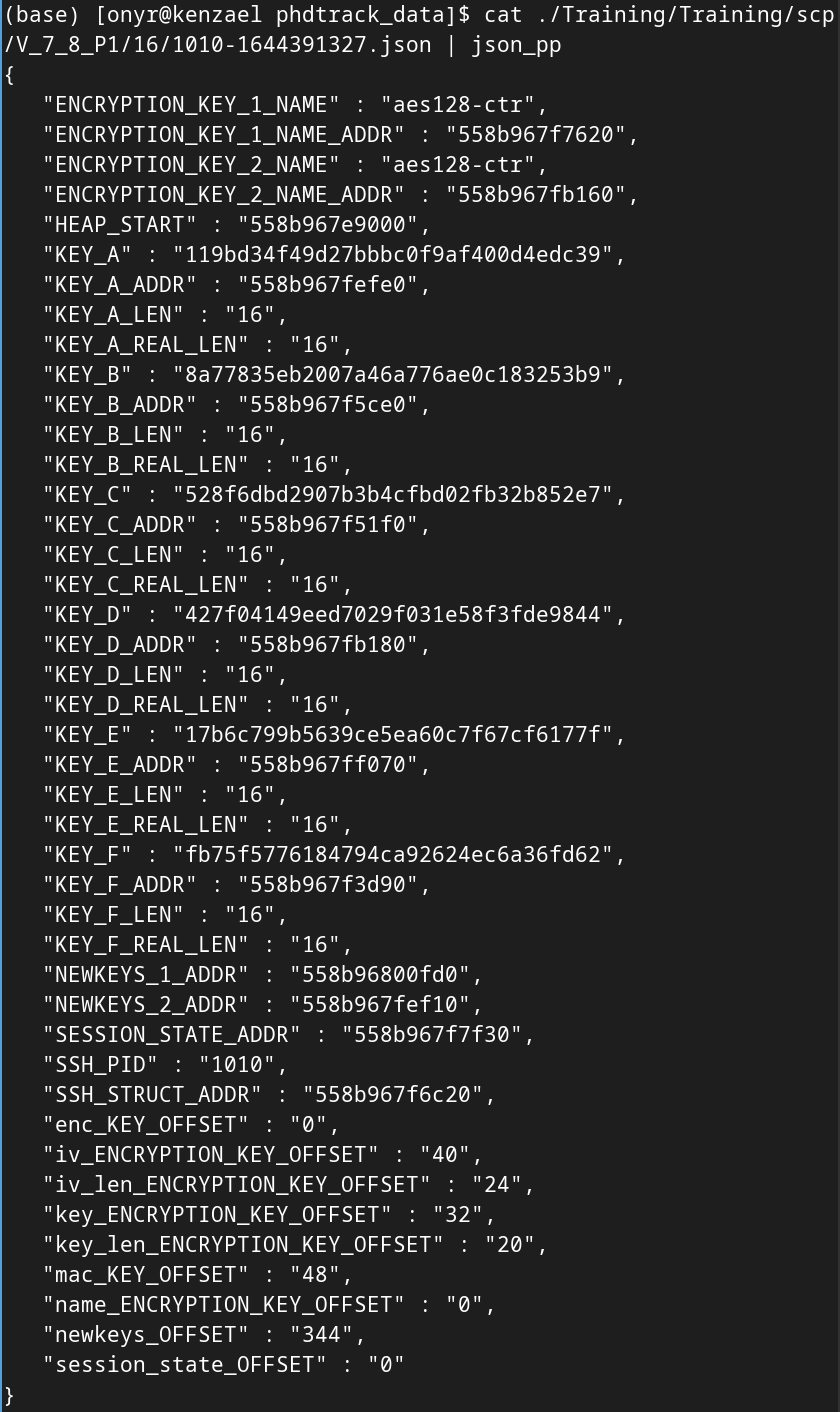
\includegraphics[width=0.6\textwidth]{img/background/json_annotation_for_1010-1644391327.png}
            \caption{Json exemple}
            \label{fig:Background:json}
        \end{figure}

        \begin{figure}[H]
            \centering
            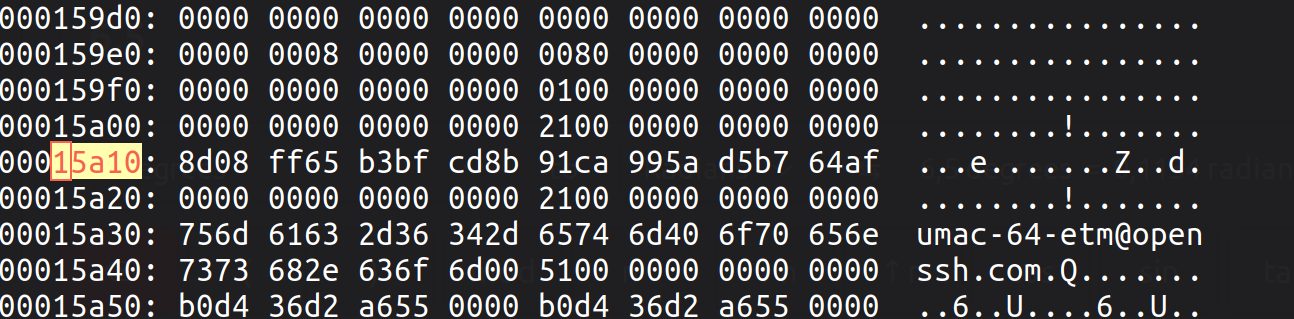
\includegraphics[width=0.6\textwidth]{img/background/xxd.png}
            \caption{Xxd exemple}
            \label{fig:Background:xxd}
        \end{figure}

        \paragraph{}The dataset is structured into two primary directories: \texttt{training} and \texttt{validation}. Each of these directories is further segmented into subdirectories reflecting the specific scenario, such as OpenSSH, port-forwarding, or secure copy (\acrshort{scp}).

        \paragraph{}Subdirectories under OpenSSH or SCP are categorized based on the software version responsible for the memory dump. These directories are further organized by the software version that generated the memory dump. The heaps are then classified based on their key lengths, with each key length possessing its dedicated directory beneath the version directory. These version-specific directories are further divided based on the different key lengths present in a heap.

        \paragraph{}Accompanying every raw memory dump is a JSON file, distinguished by the same alphanumeric sequence, barring the ``-heap'' suffix. This JSON file encapsulates various encryption keys and additional metadata, such as the process ID and the offset of the heap. Consequently, the dataset's utility is not confined to extracting session keys but also extends to identifying crucial data structures harboring sensitive information. The dataset, along with the associated code and tools, is open-sourced. The dataset is accessible via a Zenodo repository\footnote{\url{https://zenodo.org/record/6537904}}. The code can be found in a public GitHub repository\footnote{Link to the GitHub repository}.}
        
        \paragraph{}This data is the same as the data used in the paper titled \citetitle*{fellicious_smartkex_2022} \cite{fellicious_smartkex_2022}.
    
    \subsubsection{Entropy's Role in SSH Key Identification}

        \paragraph{}Encryption keys\cite*{fellicious_smartkex_2022} inherently consist of predominantly random byte sequences. This characteristic stems from the foundational principle of ensuring security through transparency, which guarantees their high entropy. The paper explores the nuances of pinpointing these keys in memory dumps, underscoring the significance of entropy in this endeavor. This particularity can be used to identify the keys in the memory dump.
        
    \subsubsection{Definitions : Structures, Pointers, and the role of malloc headers}
    
        \paragraph{}Through the use of the regular expressions (\acrshort{regex}) \texttt{"[0-9a-f]\{12\}0\{4\}"}, we identified potential \glspl{pointer} within the dump. This heuristic approach acts as a sieve, filtering the extensive data to spotlight possible \gls{pointer} candidates. Nonetheless, it's crucial to understand that while many \glspl{pointer} might be correctly pinpointed, some detected sequences may not be authentic \glspl{pointer}.

        \paragraph{}One notable characteristic of the heap dump is the \textit{malloc header} found at the start of allocated \glspl{structure}. This header, often the initial non-null bytes in a series, signifies the size of the following \gls{structure}. By sequentially reading the heap dump and identifying these headers, it becomes feasible to determine the dimensions and limits of every allocated \gls{structure}, thereby methodically dividing the heap dump into distinct \glspl{structure}.
        
\subsection{Traditional Statistical Embedding}

    \paragraph{}Within the domain of machine learning, how data is represented significantly impacts the performance of models. Even though traditional statistical embedding techniques have been around before many contemporary methods, they continue to be vital in readying data for machine learning endeavors. Rooted in statistical foundations, these techniques provide a methodical approach to transform raw data into concise and meaningful forms. In this subsection, we'll delve into the nuances of entropy and its role in byte sequence embedding, \acrfull{bfd}, and also highlight other classical statistical embedding methods pivotal in data representation for machine learning.
        
    \subsubsection{Entropy and its application in byte sequence embedding}
        \paragraph{}Entropy, a fundamental concept in information theory, quantifies the amount of uncertainty or randomness associated with a set of data. Introduced by Claude Shannon in his groundbreaking work \cite{shannon_mathematical_1948}, entropy serves as a measure of the average information content one can expect to gain from observing a random variable's value.

        \paragraph{}Mathematically, the entropy \(H(X)\) of a discrete random variable \(X\) with possible values \newline \(\{x_1, x_2, \ldots, x_n\}\) and probability mass function \(P(X)\) is given by:
        \begin{align}
            H(X) &= -\sum_{i=1}^{n} P(x_i) \log_2 P(x_i)
            \label{eq:shannon_entropy}
        \end{align}

        \paragraph{}Within the scope of identifying SSH keys, the significance of entropy cannot be understated. Byte sequences exhibiting high entropy typically reflect a multifaceted and varied informational content, traits that are synonymous with encryption keys, especially those in SSH. Sequences with pronounced entropy are often prime contenders for SSH keys due to their inherent randomness and lack of predictability, mirroring the attributes of robust security keys.

        \paragraph{}Fundamentally, entropy acts as a quantitative tool to evaluate the depth of information within data. When applied to SSH, it suggests that data sequences with elevated entropy levels have a heightened probability of correlating with secure keys. This positions entropy as an essential instrument for pinpointing and authenticating SSH keys.
    \subsubsection{Byte Frequency Distribution (BFD)}
        \paragraph{}In the complex world of raw byte embedding, \acrfull{bfd} and n-gram embedding stand out as essential methods, each bringing unique benefits to data representation. \acrshort{bfd} zeroes in on the distribution of individual byte values in a raw byte sequence. Analyzing these distributions allows for the identification of patterns that reflect the inherent nature of the data. This embedding technique becomes particularly relevant when assessing the randomness or structure of byte sequences, such as when detecting encrypted data or pinpointing specific file signatures.

        \paragraph{}On the other hand, n-gram embedding dives deeper into raw byte sequences. Instead of focusing solely on individual bytes, it captures patterns formed by sequences of 'n' consecutive bytes. This approach garners a wider range of contextual information from the raw byte data. For example, a trigram (3-gram) examines patterns formed by three sequential bytes, providing a richer representation than single byte values. Yet, a challenge with n-gram embedding is the potential for the output vector size to grow exponentially as 'n' increases, posing computational and storage issues, especially in real-time scenarios.
        
        \paragraph{}In the realm of raw byte embedding, both \acrshort{bfd} and n-gram techniques offer invaluable perspectives. While \acrshort{bfd} establishes a base representation centered on individual byte frequencies, n-gram embedding enhances it by spotlighting the complex relationships and patterns among consecutive bytes. Together, they form a robust arsenal for representing and analyzing raw byte data in a variety of applications.
    \subsubsection{Other traditional statistical embedding techniques}
        \paragraph{Mean Byte Value}The Mean Byte Value represents the average value of all bytes in a given sequence. It provides an insight into the central tendency of the byte values in the sequence. Mathematically, for a byte sequence \( B \) of length \( n \):
        \begin{equation}
        \text{Mean Byte Value} = \frac{1}{n} \sum_{i=1}^{n} B_i
        \label{eq:mean_byte_value}
        \end{equation}

        \paragraph{Mean Absolute Deviation (MAD)}MAD measures the average distance of each byte value from the mean, providing a sense of the dispersion or spread of the byte values around the mean. It is given by:
        \begin{equation}
        \text{MAD} = \frac{1}{n} \sum_{i=1}^{n} |B_i - \text{Mean Byte Value}|
        \label{eq:mad}
        \end{equation}

        \paragraph{Standard Deviation}Standard Deviation quantifies the amount of variation or dispersion in the byte sequence. A higher value indicates greater variability in the byte values. It is defined as:
        \begin{equation}
        \text{Standard Deviation} = \sqrt{\frac{1}{n} \sum_{i=1}^{n} (B_i - \text{Mean Byte Value})^2}
        \label{eq:standard_deviation}
        \end{equation}

        \paragraph{Skewness}Skewness\cite{wheeler_problems_2011} measures the asymmetry of the distribution of byte values around the mean. A positive value indicates a distribution that is skewed to the right, while a negative value indicates a distribution skewed to the left. It provides insights into the shape of the distribution of byte values. The Fisher’s skewness\cite{cain_univariate_2017} is :
        \begin{equation}
        \text{Skewness} = \frac{n}{(n-1)(n-2)} \sum_{i=1}^{n} \left( \frac{B_i - \text{Mean Byte Value}}{\text{Standard Deviation}} \right)^3
        \label{eq:skewness}
        \end{equation}

        \paragraph{Kurtosis}Kurtosis\cite{wheeler_problems_2011} measures the "tailedness" of the distribution of byte values. A higher kurtosis value indicates a distribution with heavier tails, while a lower value indicates lighter tails. It provides insights into the extremities of the distribution. The Fisher’s kurtosis\cite{cain_univariate_2017} is :
        \begin{equation}
        \text{Kurtosis} = \frac{n(n+1)}{(n-1)(n-2)(n-3)} \sum_{i=1}^{n} \left( \frac{B_i - \text{Mean Byte Value}}{\text{Standard Deviation}} \right)^4 - \frac{3(n-1)^2}{(n-2)(n-3)}
        \label{eq:kurtosis}
        \end{equation}

        \paragraph{n-gram on Bits}When applying n-gram techniques to bits instead of bytes, we focus on sequences of 'n' consecutive bits. For example, a 2-gram on bits would consider patterns formed by two consecutive bits, resulting in four possible combinations: 00, 01, 10, and 11. This approach significantly reduces the size of the output vector compared to byte-based n-grams. By focusing on bits, we can capture more granular patterns in the data while benefiting from a more compact representation, which is computationally efficient and requires less storage.

\subsection{Deep Learning Models for Raw Byte Embedding}

    \paragraph{}In the area of data representation, deep learning is great for understanding raw byte sequences. Just like these models are good at understanding text, they're also good at understanding raw bytes. They can learn and show sequences on their own, which is really helpful for both text and raw bytes. In this section, we'll look at different deep learning models and how they work with raw byte embedding.

    \paragraph{}We'll start with \acrfull{rnn}. Just like they're good with word sequences in text, \acrfull{rnn} are also good with raw byte sequences. Then, we'll look at \acrfull{cnn}, which can find patterns in raw bytes, just like they find patterns in text. After that, we'll talk about Autoencoders, which can learn in a special way. To finish this section, we'll discuss Transformers. They're good at understanding data over a long time, similar to how they understand text.

    \subsubsection{RNNs : Understanding sequence data}
        \paragraph{}\acrfull{rnn} are great tools for text classification. They're good at understanding the deeper meanings in text. Unlike older models that use hand-made features, \acrshort{rnn} can learn and show sequences on their own. This makes them really useful for tasks that deal with sequences. When we think about embedding raw bytes, \acrshort{rnn}'s skill in understanding sequences is similar to how they handle word sequences in text. Here is a list of different \acrshort{rnn} models and their advantages and disadvantages.

        \paragraph{\acrfull{rcnn} for Text Classification\cite{lai_recurrent_2015}:} The \acrshort{rcnn} model, as discussed in the paper by Lai et al., is designed specifically for text classification. Unlike traditional models, \acrshort{rcnn} do not rely on handcrafted features. Instead, they employ a recurrent structure to capture contextual information about words. This approach is believed to introduce considerably less noise compared to traditional window-based neural networks. The model's bidirectional structure ensures that both preceding and succeeding contexts of a word are considered, enhancing its understanding of the word's semantics.

        \begin{itemize}
            \item \textbf{Advantages:} 
            \begin{itemize}
                \item No need for handcrafted features.
                \item Captures richer contextual information.
                \item less noisy.
            \end{itemize}
            \item \textbf{Disadvantages:} 
            \begin{itemize}
                \item Complexity due to bidirectional structure.
                \item Might require more computational resources.
            \end{itemize}; 
        \end{itemize}

        \paragraph{\acrfull{lstm}\cite{hochreiter_long_1997}:}The \acrshort{lstm}, introduced by Hochreiter and Schmidhuber, is a specialized form of \acrshort{rnn} designed to combat the vanishing gradient problem inherent in traditional \acrshort{rnn}. The vanishing gradient problem arises when gradients of the loss function, which are used to update the network's weights, become too small for effective learning. This typically happens in deep networks or when processing long sequences, causing the earlier layers or time steps to receive minimal updates. As a result, traditional \acrshort{rnn} struggle to learn long-term dependencies in the data.

        \paragraph{}\acrshort{lstm} address this issue with their unique cell state and gating mechanisms. The cell state acts as a "conveyor belt" that can carry information across long sequences with minimal changes, ensuring that long-term dependencies are captured. The gating mechanisms, namely the input, forget, and output gates, regulate the flow of information into, out of, and within the cell. This design allows LSTMs to selectively remember or forget information, making them adept at learning and retaining long-term dependencies in sequences.

        \begin{itemize}
            \item \textbf{Advantages:}
            \begin{itemize}
                \item Efficiently learns long-term dependencies; overcomes the vanishing gradient problem inherent in traditional \acrshort{rnn}.
                \item Often achieves faster and more stable learning.
            \end{itemize}
            \item \textbf{Disadvantages:}
            \begin{itemize}
                \item More complex architecture compared to basic \acrshort{rnn} and even \acrshort{gru}.
                \item Can be computationally intensive due to the multiple gating mechanisms.
            \end{itemize}
        \end{itemize}

        \paragraph{\acrfull{gru}\cite{chung_empirical_2014}:} \acrshort{gru} are a variant of \acrshort{rnn} that aim to capture long-term dependencies without the complexity of \acrshort{lstm}. They use a gating mechanism to control the flow of information, making them efficient in sequence modeling tasks.

        \begin{itemize}
            \item \textbf{Advantages:} 
            \begin{itemize}
                \item Simplified structure compared to \acrshort{lstm}.
                \item Efficient in capturing long-term dependencies.
                \item Sometimes outperforms \acrshort{lstm}.
            \end{itemize}
            \item \textbf{Disadvantages:} 
            \begin{itemize}
                \item Still more complex than traditional \acrshort{rnn}.
                \item Might not always outperform \acrshort{lstm} in all tasks.
            \end{itemize}
        \end{itemize}
        

        \paragraph{}To sum it up, \acrshort{rnn} are good at understanding sequences and context. This makes them a good choice for embedding raw bytes. Just like they understand words based on the words around them, \acrshort{rnn} can find patterns in raw byte sequences, giving us a better understanding of the data.
    \subsubsection{CNNs : Pattern detection in raw bytes}
        \paragraph{}\acrfull{cnn}\cite{lecun_gradient-based_1998} are a specialized category of deep learning models adept at identifying patterns. Originally designed for visual data, their prowess extends to tasks like image and document recognition. Drawing inspiration from the human visual cortex's biological processes, \acrshort{cnn} are architected to autonomously and adaptively discern spatial feature hierarchies from inputs. This becomes particularly relevant when considering raw byte embedding, where the goal is to detect patterns in sequences of bytes. The CNN architecture boasts convolutional layers that perform operations on input data to capture localized patterns, and pooling layers that condense spatial dimensions while preserving crucial information. This layered approach enables \acrshort{cnn} to detect intricate patterns by progressively building on simpler foundational patterns. When applied to byte sequences or document recognition, \acrshort{cnn} excel, showcasing remarkable efficacy, especially in tasks like identifying patterns within raw byte sequences or recognizing handwritten content.

        \paragraph{}When tailored to \acrshort{cnn}, the \acrfull{seq2seq}\cite{gehring_convolutional_2017} approach emerges as a potent tool for transforming raw byte sequences into meaningful embeddings. The encoder segment of the \acrshort{seq2seq} model is central to this transformation. It delves into the byte sequence, discerning intricate patterns and nuances, and distills this rich information into a concise context vector or embedding. This condensed representation captures the core essence of the byte sequence, positioning it as a valuable input for subsequent tasks, such as classification models.

        \paragraph{}At the heart of the encoder lie the convolutional layers, skilled in pinpointing specific patterns within the byte sequence. Whether it's unique byte combinations or indicative n-grams, these layers are primed to detect them. As they traverse the raw byte sequence, they employ specialized filters, honed to recognize these specific patterns. As the data flows through the encoder's layers, these identified patterns are synthesized and refined, culminating in a comprehensive embedding of the sequence.

        \paragraph{}Here are two \acrfull{seq2seq} models using \acrshort{cnn} :
        

        \begin{itemize}
            \item \textbf{Autoencoders:} These neural network architectures\cite{hinton_reducing_2006} are designed for data compression and reconstruction. The encoder part compresses the input data into a compact representation, while the decoder reconstructs the original data from this representation. In the context of raw byte sequences, the encoder can be used to generate embeddings that capture the essential patterns and structures of the data.

            \item \textbf{Transformers :} Transformers\cite{vaswani_attention_2017} utilize self-attention mechanisms to weigh the significance of different parts of the input data. This allows them to capture long-range dependencies and relationships in the data. When applied to raw byte sequences, transformers can generate embeddings that consider both local and global patterns, making them particularly effective for tasks that require understanding the broader context of a sequence.

        \end{itemize}
        
        \paragraph{}Yet, a significant challenge with traditional \acrfull{seq2seq} models using \acrshort{cnn} is their constraint in managing inputs of varying sizes. Constructed with a set input size, they face difficulties when presented with sequences of diverse lengths, like raw byte sequences.

        \paragraph{}To address this limitation, various techniques have been employed to normalize the size of the input data. One of the most common methods is \textbf{padding}, where shorter sequences are filled with predefined placeholder values (often zeros) until they match the length of the longest sequence in the dataset. This ensures that all sequences fed into the model have a uniform length. Another approach is \textbf{bucketing}, where sequences of similar lengths are grouped together, minimizing the amount of padding required. Additionally, \textbf{truncation} can be used to shorten sequences that exceed a certain length, although this might result in the loss of some information. While these techniques enable \acrshort{cnn}-based \acrfull{seq2seq} models to handle variable-sized inputs, it's crucial to ensure that the preprocessing steps do not introduce noise or distort the inherent patterns and relationships within the raw byte sequences.
\subsection{Graph Embedding Methods}
    Wait Onyr

\subsection{Machine learning}
    \paragraph{}Machine learning, an integral part of artificial intelligence, revolves around designing algorithms and statistical models that allow computers to perform tasks without being directly programmed. Instead of relying on detailed instructions for every task, machine learning techniques empower systems to learn from data and make data-driven decisions. A key method in this field is supervised learning, in which models are trained using data that comes with predefined labels. Here, each piece of data in the training set has an associated known output. The primary goal of supervised learning is to establish a relationship between inputs and outputs, enabling the model to predict or categorize new, unseen data based on this relationship.

    \paragraph{}A cornerstone in this realm is feature engineering, which involves the meticulous process of selecting and transforming variables to optimize model performance. Another challenge frequently encountered by practitioners is dealing with datasets where some classes are overrepresented, which can skew model predictions. Among the myriad of machine learning models available, certain ones have gained prominence due to their versatility and effectiveness. We will provide an overview of some of these notable models.
\section{Methods}\label{chap:methods}
    \paragraph{}This research dives into the complexities of embedding byte sequences, focusing particularly on the extraction of structures containing SSH keys for machine learning purposes. The varied uses of OpenSSH introduce distinct challenges due to potential variations in the created embeddings. Given the wide array of SSH key dimensions and OpenSSH's intricate operations, maintaining the embeddings' stability and consistency is vital. In this methodological section, we will detail various embedding methods, present a framework for their assessment through a classifier model, and suggest another strategy to verify the embeddings' coherence between the different OpenSSH usage and key sizes.

    
    \subsection{Embeddings}
    \paragraph{}From the Zenodo dataset\ref{seq:background:dataset}, we've isolated distinct memory structures within the raw heap dump files. These structures possess diverse sizes, necessitating the use of an embedding method for classification. Fortunately, a distinguishing feature of each memory structure is the presence of a header, containing vital information such as the structure's size in bytes. To precisely pinpoint the boundaries of each memory structure, we sequentially parse through the raw heap dump files. Beginning the parsing process from the first non-null byte, identified as the header, serves as a marker for the initiation of a new structure. The size data within this header is then leveraged to calculate the exact length of the structure, allowing for the extraction of its entire raw byte data while determining the start of the subsequent one.
    
    \paragraph{}Our next objective centers on the conversion of raw byte data into fixed-size embeddings (\ref{seq:background:traditional_statistical_embedding}, \ref{seq:background:deep_learning_models_for_raw_byte_embedding}), a pivotal step in preparing them for utilization in machine learning applications. Ensuring uniformity in embedding size across all memory structures holds paramount significance. Consistency in embedding dimensions is vital to empower machine learning algorithms for efficient data processing and analysis. This uniformity not only simplifies the integration of memory structures with varying sizes into a coherent classification framework but also acts as a defense against the adverse effects of the curse of dimensionality—a phenomenon that can introduce computational complexities and heighten the risk of overfitting in high-dimensional data spaces. Striking this equilibrium is essential, achieved by maintaining reasonably low embedding dimensions, fostering both efficient data processing and the preservation of essential information within the raw byte data. Additionally, it's worth noting that we will explore various embedding methods to optimize performance.

    \subsection{Embedding quality}
    \paragraph{} Transitioning our focus, we now delve into evaluating the quality of the embeddings. The dataset is notably imbalanced \ref{seq:background:imbalanced_data}, primarily stemming from the rarity of memory structures containing SSH keys, our specific target of interest, within the overall dataset. This rarity results in a significant class imbalance, where the majority of memory structures do not contain SSH keys. To counteract potential bias toward the majority class, we will implement the \acrfull{smote} as a resampling strategy, enabling our model to accurately classify both majority and minority classes. We will then employ a Random Forest model \ref{seq:background:machine_learning}, renowned for its robustness and suitability for high-dimensional data, to carry out the classification task. Our evaluation will rely on metrics such as precision, recall, F1 score, and others to identify the most effective representation for precise classification.

    \subsection{Embedding coherence}
\chapter{Results}\label{chap:results}

\paragraph{}In this thesis, we undertake a thorough investigation of data embeddings and their effectiveness in predicting SSH keys within OpenSSH memory dumps. The results are methodically structured, starting with Data Preprocessing, where we lay a solid foundation by preparing the data for in-depth analysis. We proceed to evaluate Deep Learning Models, analyzing their architecture and limitations. This is succeeded by Feature Engineering, where we meticulously refine our data to improve model accuracy. Through Clustering analysis, we explore and identify underlying patterns within the data. Ultimately, we employ Classification techniques to accurately predict and categorize SSH keys, thus demonstrating the practical implications and utility of our research. 
    

\section{Data Preprocessing}

\paragraph{}In the data preprocessing stage, we meticulously calculated each embedding four times, which included the deep learning models. This repetition was to test all combinations of the two filters—entropy and chunk size. The purpose of this thorough approach was to discern the effectiveness of each filter, both individually and in combination, providing us with a clearer understanding of their impact on the data and the subsequent results. The different datasets used are detailed in Section \ref{sec:annexe:all_dataset}. The dataset codes are explained in the following table~\ref{tab:results:dataset_codes}:

\begin{table}[ht]
    \centering
    \begin{tabular}{|p{0.3\linewidth}|p{0.6\linewidth}|}
    \hline
    Dataset Code & Meaning \\ 
    \hline
    value\_node\_embedding & First graph embedding, with all nodes~\ref{sec:embedding:first_graph} \\ \hline
    chunk\_top\_vn\_semantic\_embedding & First graph embedding, keeping only the first block of each chunk~\ref{sec:embedding:first_graph_only_first_block} \\ \hline
    chunk\_semantic\_embedding & Second graph embedding~\ref{sec:embedding:updated_graph} \\ \hline
    chunk\_statistic\_embedding & Statistical embedding~\ref{sec:embedding:statistical} \\ \hline
    chunk\_start\_bytes\_embedding & Start bytes embedding~\ref{sec:embedding:trim_method} \\ \hline
    chunk\_extraction & Raw byte extraction with filters, to be fed into the deep learning model\\ \hline
    \end{tabular}
    \caption{Meanings of Dataset Codes}
    \label{tab:results:dataset_codes}
\end{table}


\section{Deep Learning Models}

\paragraph{}The exploration of hyperparameters is documented in Section \ref{sec:annexes:deep_learning_hyperparameters}. During our experiments, we encountered instances where some models either ran out of memory, as noted in Sections \ref{sec:annexe:out_of_memory_instances_classifications} and \ref{sec:annexe:out_of_memory_instances_clustering}, or experienced timeouts, detailed in Section \ref{sec:annexe:timeout_instances}. Consequently, our discussion will be confined to the results yielded by the models that successfully completed their runs.

\paragraph{}Within the cohort of operational deep learning models, we endeavored to identify the most proficient instance for each algorithm, whether it was Transformers or Word2Vec. However, we encountered a scarcity of successful instances, which impeded our ability to conclusively determine the optimal hyperparameters or to fully understand their impact on the classification metrics. It was observed that instances with a larger word size and a reduced embedding dimension were more likely to succeed, presumably due to the decreased computational load they required.

\section{Feature Engineering}
\paragraph{}During our feature engineering phase, we encountered a challenge that led to the elimination of certain embeddings. This was due to the invariance observed in the columns, an issue that is elaborated upon in Section \ref{sec:annexe:feature_engineering_fails}. The specific embedding that was rendered ineffective and subsequently removed was the semantic embedding of the first graph, as discussed in Section \ref{sec:embedding:graph_embedding}. This elimination was necessary regardless of whether the filter on the first block of each chunk was applied. The primary shortcoming of this embedding was its inability to generate a sufficient number of ancestors to provide useful information. This inadequacy arose because only a minor segment of the value nodes were being pointed to by pointers, which significantly limited the utility of the embedding. In contrast, the second graph managed to compress the information effectively, thereby validating the semantic embedding by conveying more meaningful data for each node.

\paragraph{}The instances that successfully passed the feature engineering stage are meticulously recorded in Section \ref{sec:annexe:feature_engineering_results}. Here, the eight most significant columns are identified.

\section{Clustering}
\paragraph{}In the clustering phase of our analysis, we categorized the data into distinct groups: label 1 for SSH keys, label 2 for "ssh\_struct", label 4 for "session\_state\_struct", and label 0 for the remainder. The detailed outcomes of this clustering are presented in appendix \ref{sec:annexe:clustering_results}. Our examination revealed that the majority of clusters did not exhibit discernible patterns. However, certain datasets, such as those represented by chunk\_start\_bytes\_embedding (23) in Table \ref{tab:23_single_instance_clustering_results} and chunk\_statistic\_embedding (18) in Table \ref{tab:18_single_instance_clustering_results}, maintained a ratio of labels similar to that of the original dataset.


\paragraph{}Interestingly, the clusters derived from deep learning models typically displayed an even distribution of labels, with approximately one quarter of the data falling into each category. An exception to this trend was observed in the Word2Vec 3 Clustering Results on dataset 25 (with chunk size filter), as shown in Table \ref{tab:25_word2vec_3_clustering_results}, which consisted of three clusters with seemingly random label proportions.

\paragraph{}The results from the clustering analysis were not entirely definitive, indicating that there is substantial room for improvement in the methodology. Future efforts in this area would benefit from a more refined approach to enhance the clarity and significance of the clustering outcomes.

\section{Classification}

\paragraph{}The classification results of our study, detailed in appendix \ref{sec:annexe:classification_results}, yielded highly promising results. The performance of various instances, particularly in terms of accuracy, is depicted in the graphical representation found in Figure \ref{fig:results:best_accuracy_instances}, which ranks the instances from best to worst.

\begin{figure}[ht]
    \centering
    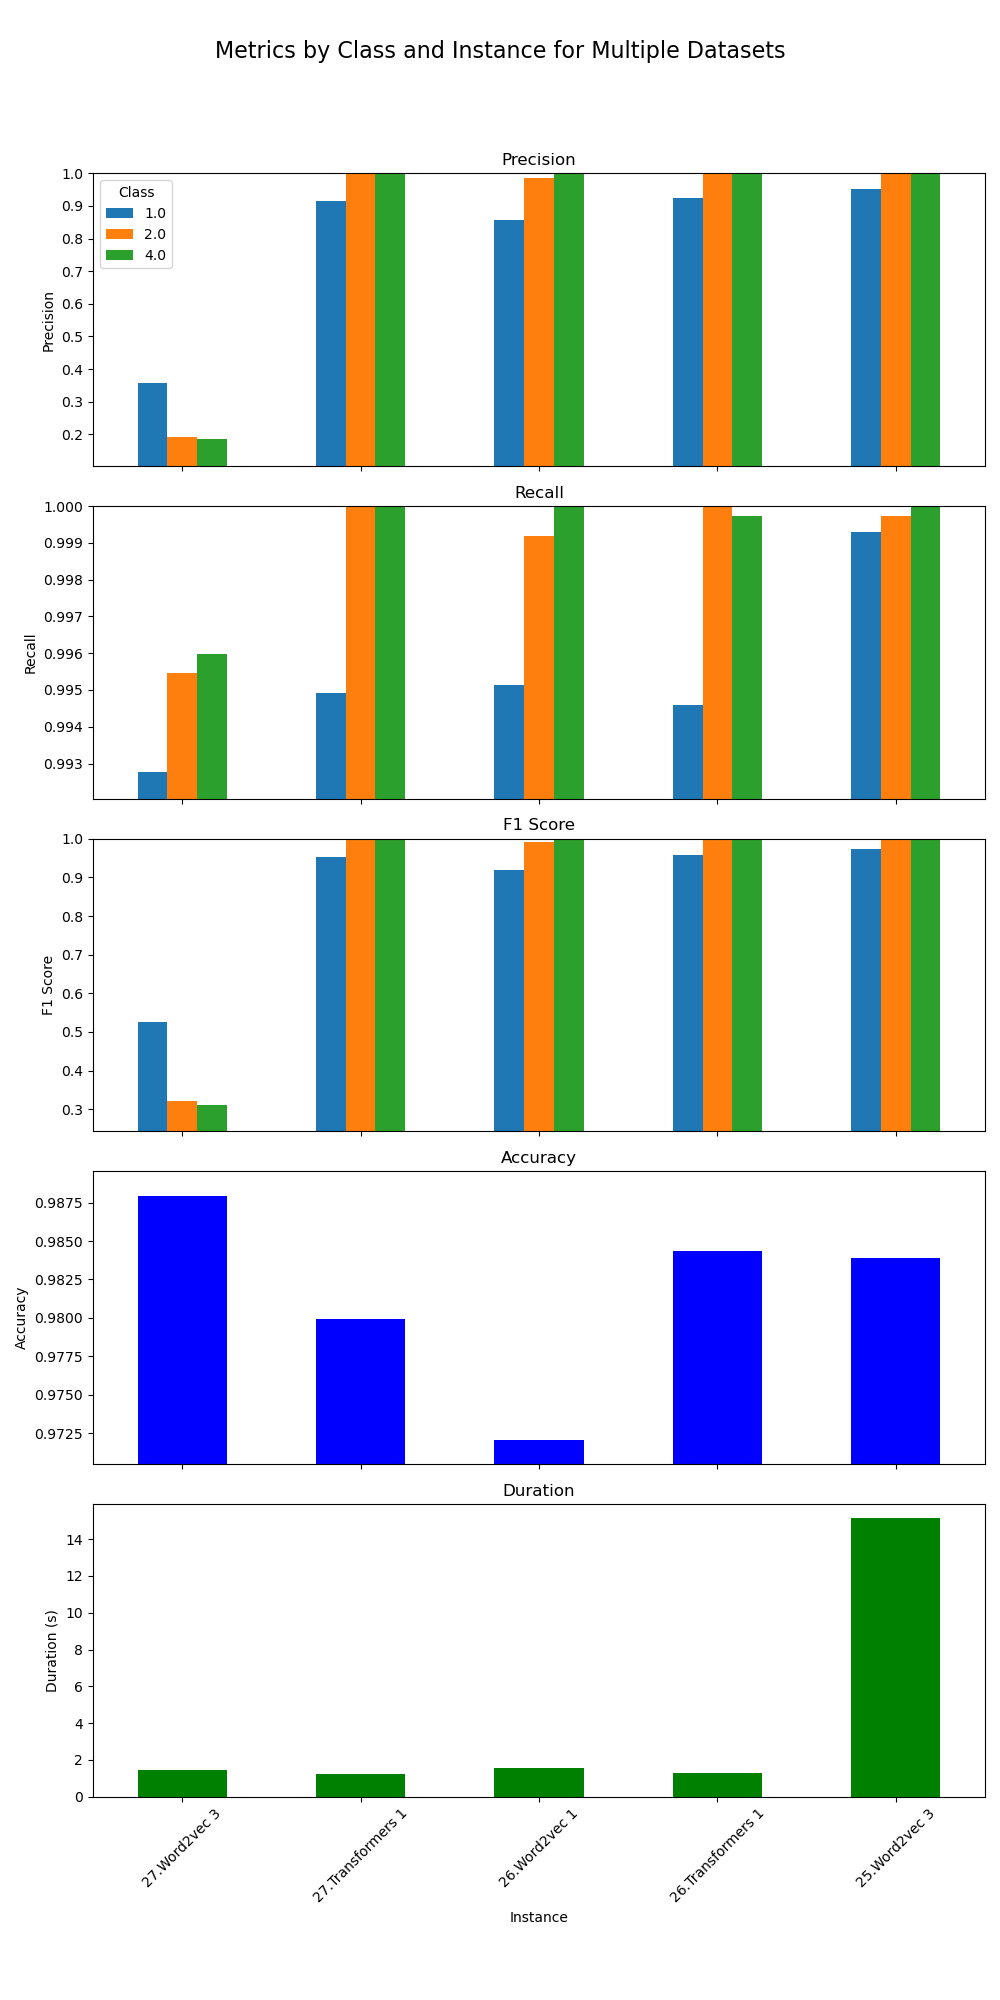
\includegraphics[width=0.6\textwidth]{img/annexes/Best Accuracy (by instances).png}
    \caption{Metrics for the best instances (accuracy)}
    \label{fig:results:best_accuracy_instances}
\end{figure}

\paragraph{}The two top-performing instances, both utilizing chunk\_start\_bytes\_embedding, achieved remarkable accuracy scores of 99.90\% with the chunk size filter~\ref{tab:21_single_instance_classifiers_results} and 99.84\% without the filter~\ref{tab:20_single_instance_classifiers_results}. Following closely was chunk\_semantic\_embedding with the chunk size filter, securing an accuracy of 99.70\%~\ref{tab:9_single_instance_classifiers_results}. Notably, the first deep learning model to make an appearance in the ranking was a Word2Vec model, which, with both entropy and chunk size filters applied, attained an accuracy of 98.79\%, placing it sixth overall~\ref{tab:27_word2vec_3_classifiers_results}.

\paragraph{}When focusing on recall for label 1, the best instance was chunk\_start\_bytes\_embedding without any filter, achieving a perfect recall of 100\%~\ref{tab:20_single_instance_classifiers_results}, as shown in Figure \ref{fig:results:best_label_1_recall_instances}. The second-best was again chunk\_start\_bytes\_embedding, this time with both entropy and chunk size filters, achieving a recall of 99.99553\%~\ref{tab:23_single_instance_classifiers_results}. The first deep learning model, a Word2Vec instance with both filters, ranked third with a recall of 99.95\%.

\begin{figure}[ht]
    \centering
    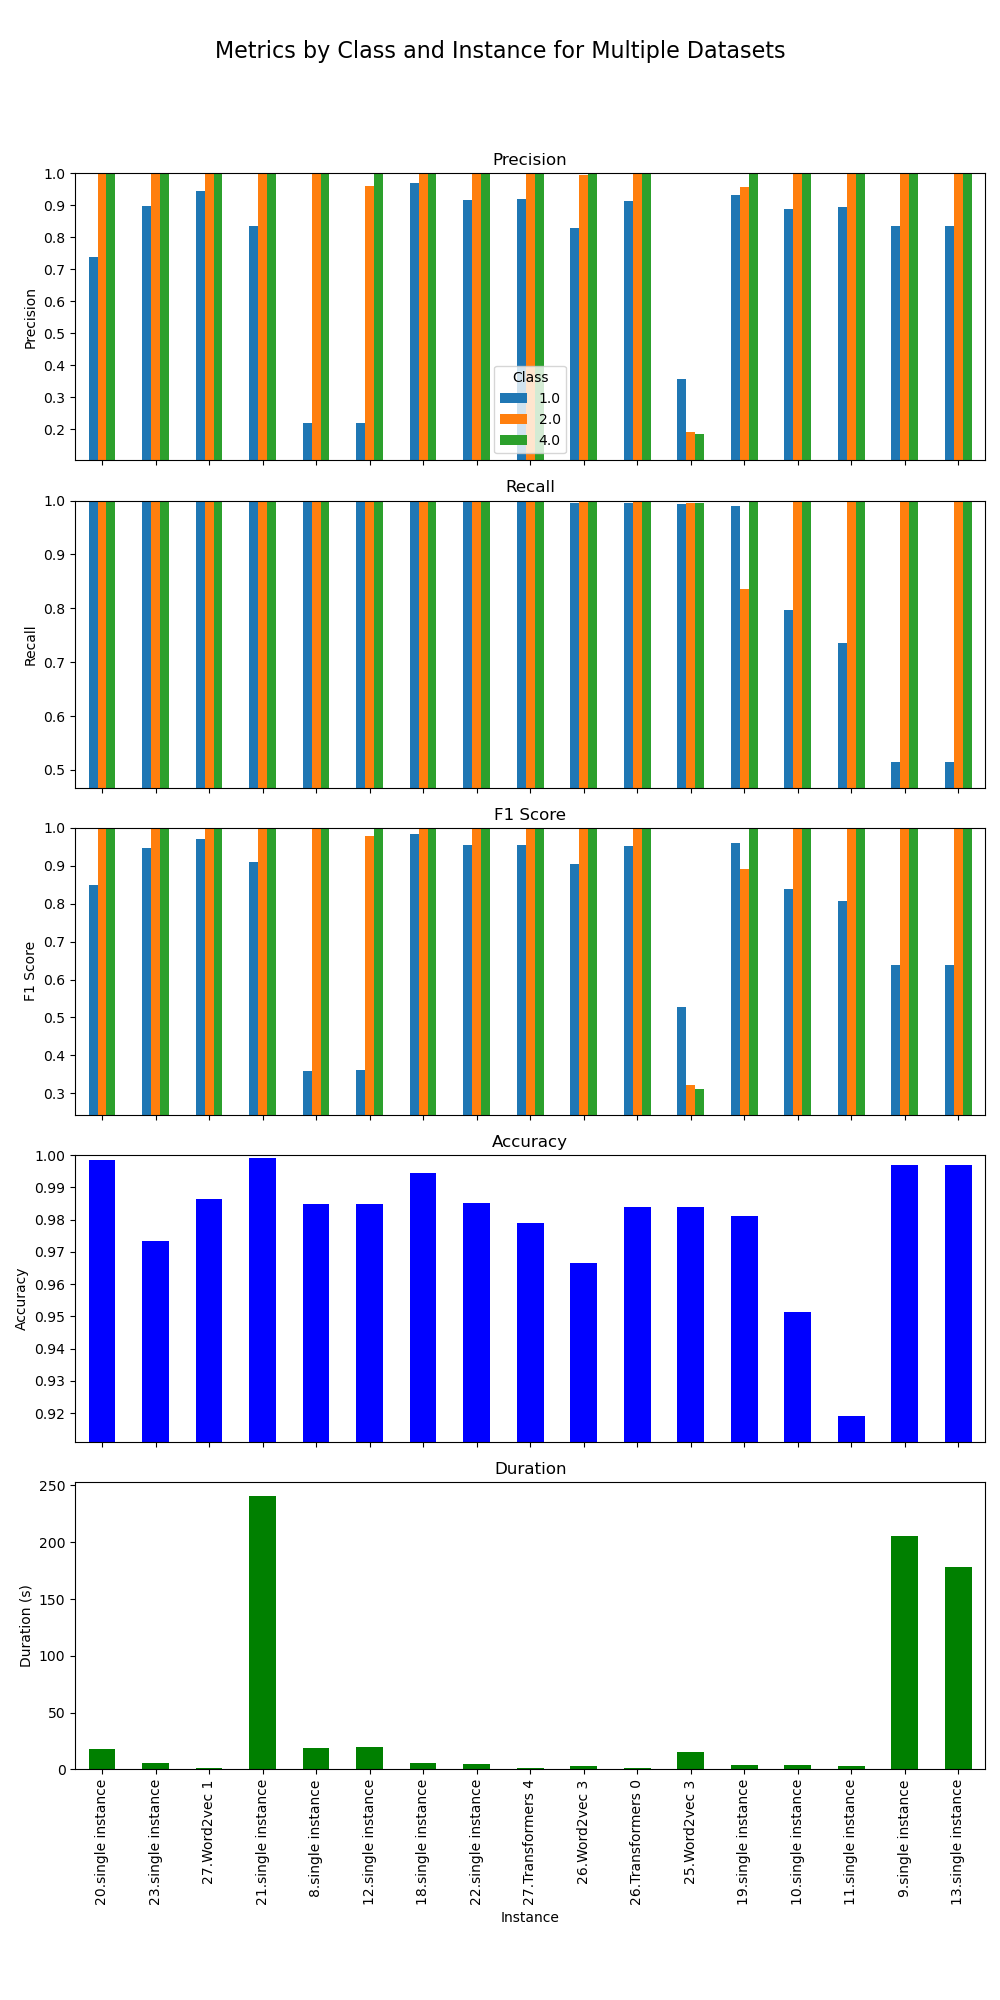
\includegraphics[width=0.6\textwidth]{img/annexes/Best 1.0 Recall (by instances).png}
    \caption{Metrics for the best instances (Label 1 recall)}
    \label{fig:results:best_label_1_recall_instances}
\end{figure}

\paragraph{}As for precision on label 1, the highest achievement was recorded by chunk\_statistic\_embedding with the entropy filter, which reached a precision of 96.86\%~\ref{tab:18_single_instance_classifiers_results}, as illustrated in Figure \ref{fig:results:best_label_1_precision_instances}. The second-highest precision came from a Word2Vec deep learning model with both entropy and chunk size filters, scoring 95.19\%.

\begin{figure}[ht]
    \centering
    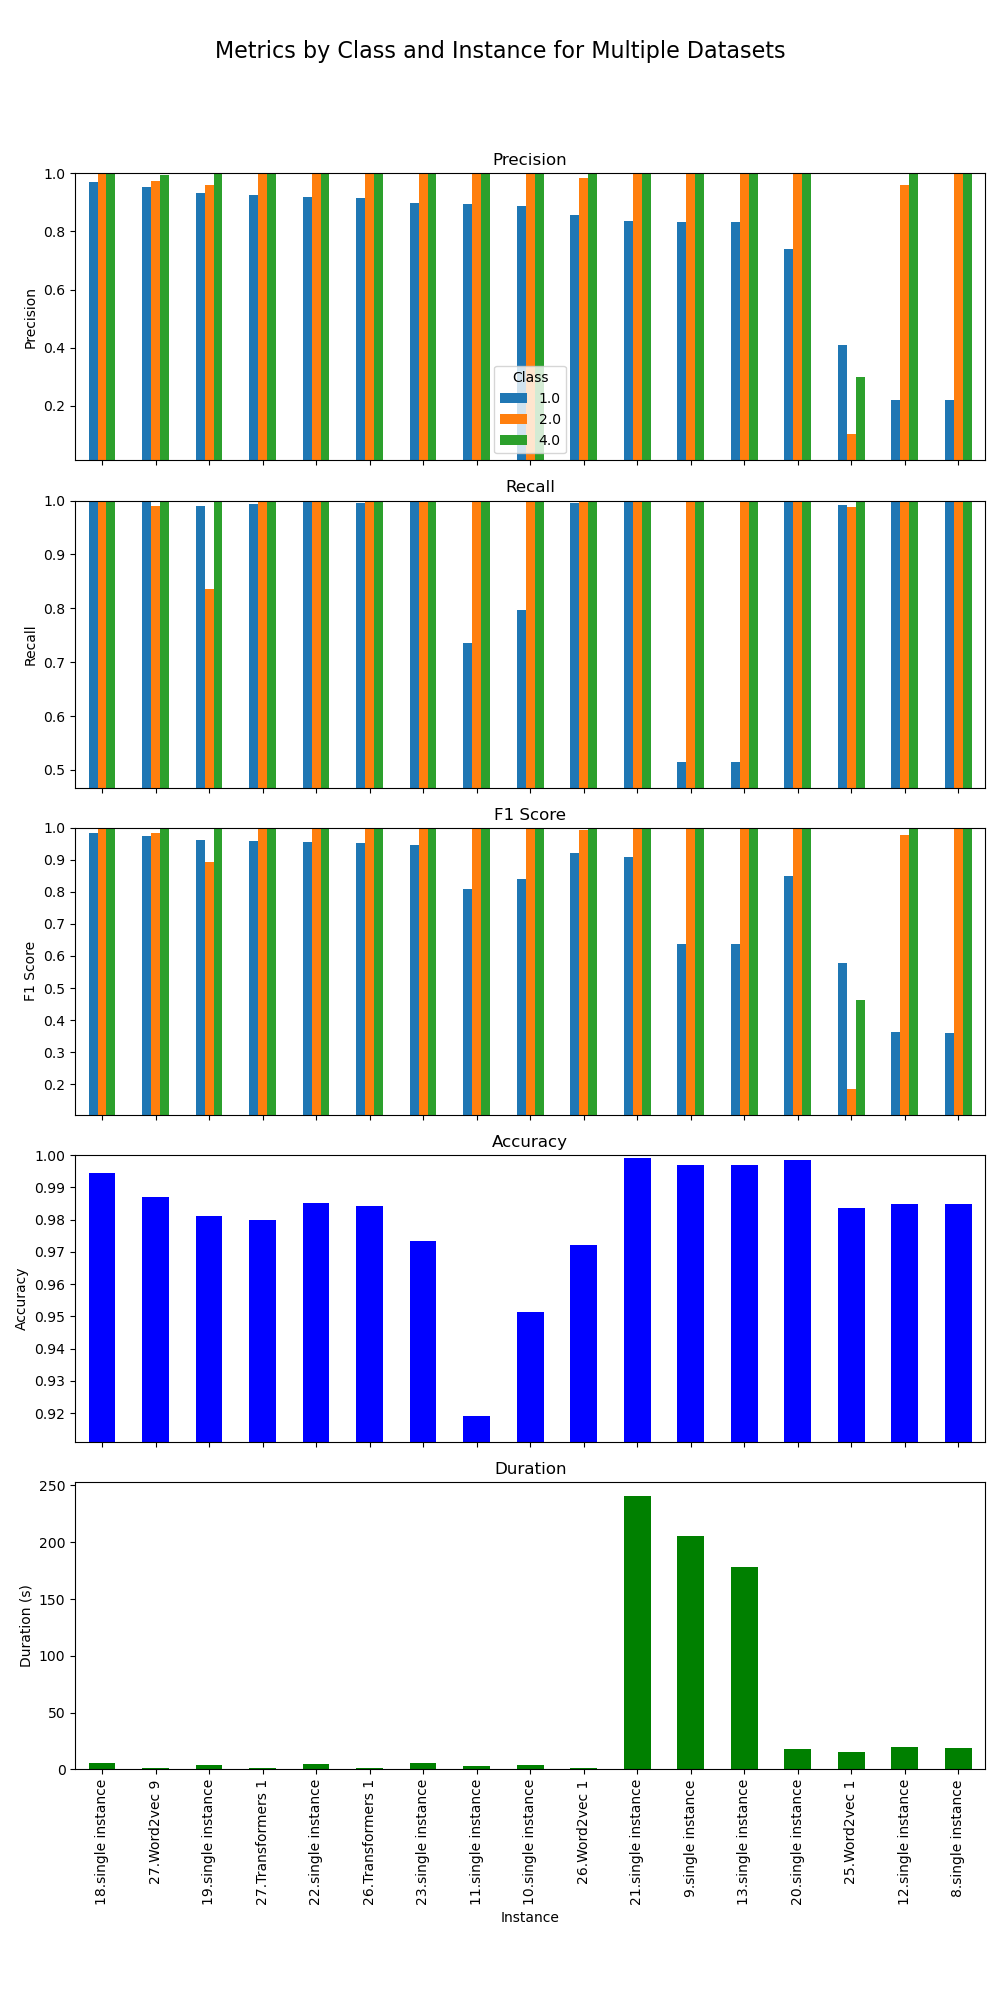
\includegraphics[width=0.6\textwidth]{img/annexes/Best 1.0 Precision (by instances).png}
    \caption{Metrics for the best instances (Label 1 precision)}
    \label{fig:results:best_label_1_precision_instances}
\end{figure}


\chapter{Discussion}\label{chap:discussion}


Discuss the results. What is the outcome of your experimetns?
\chapter{Conclusion}\label{chap:conclusion}

\paragraph{}In conclusion, this Master's thesis has provided a comprehensive survey of various embedding techniques for the classification of SSH keys in OpenSSH memory dumps. The study has uncovered that simple embedding techniques, such as the trim method and statistical approaches, yield highly effective results when applied to this specific dataset. Additionally, NLP techniques like Word2Vec and Transformers have shown promising outcomes, although they require further refinement through hyperparameter tuning to reach their full potential.

\paragraph{}While coherence testing has not been conclusively demonstrated, the classification results have been exceptionally positive, indicating the practical value of the research. However, there remains a substantial scope for future work. This includes measuring the time efficiency of the embedding processes, extensive hyperparameter optimization, exploration of additional NLP techniques, and more rigorous coherence testing. These areas present exciting opportunities for further research and development in the field of digital forensics and cybersecurity.

%%%%%%%%%%%%%%%%%%%%%%%%%%%%%%%%%%%%%%%%%%%%%%%%%%%%%%%%%%%%%%%%%%%%%%%%%%%%%%%%%%%%%%%%%
\newpage
% -- Appendix (optional)
\begin{appendices}
    % !TeX spellcheck = en\_US
% !TeX encoding = UTF-8
\chapter{Models}
\section{Machin Learning Hyperparameters}
\subsection{Random Forest Classifier}

    \begin{table}[ht]
        \centering
        \caption{Default Parameters for Random Forest Classifier}
        \begin{tabular}{lc}
            \textbf{Parameter} & \textbf{Default Value} \\
            bootstrap & True \\
            ccp\_alpha & 0.0 \\
            class\_weight & None \\
            criterion & gini \\
            max\_depth & None \\
            max\_features & sqrt \\
            max\_leaf\_nodes & None \\
            max\_samples & None \\
            min\_impurity\_decrease & 0.0 \\
            min\_samples\_leaf & 1 \\
            min\_samples\_split & 2 \\
            min\_weight\_fraction\_leaf & 0.0 \\
            n\_estimators & 100 \\
            n\_jobs & -1 \\
            oob\_score & False \\
            random\_state & 42 \\
            verbose & 0 \\
            warm\_start & False \\
        \end{tabular}
    \end{table}

    \subsection{OPTICS Clustering}

    \begin{table}[ht]
        \centering
        \caption{Default Parameters for OPTICS Clustering}
        \begin{tabular}{lc}
            \textbf{Parameter} & \textbf{Default Value} \\
            algorithm & brute \\
            cluster\_method & xi \\
            leaf\_size & 30 \\
            max\_eps & inf \\
            memory & None \\
            metric & cosine \\
            metric\_params & None \\
            min\_cluster\_size & None \\
            n\_jobs & -1 \\
            p & 2 \\
            predecessor\_correction & True \\
            xi & 0.05 \\
        \end{tabular}
    \end{table}


    \paragraph{Note for OPTICS:}
    \begin{description}
        \item[min\_samples:] Calculated dynamically for each embedding.
        \item[eps:] Takes five distinct values: 0.01, 0.02, 0.03, 0.04, and 0.05.
    \end{description}

\section{Deep learning hyperparameters}
    \subsection{Transformers:}
        \begin{table}[ht]
            \centering
            \caption{Transformers Hyperparameters (Configurations 0–4)}
            \begin{tabular}{lccccc}
                & Config 0 & Config 1 & Config 2 & Config 3 & Config 4 \\
                word character size & 16 & 16 & 8 & 8 & 16 \\
                embedding dim & 8 & 16 & 8 & 16 & 8 \\
                transformer units & 2 & 2 & 2 & 2 & 4 \\
                num heads & 2 & 2 & 2 & 2 & 4 \\
                num transformer layers & 2 & 2 & 2 & 2 & 4 \\
                dropout rate & 0.1 & 0.1 & 0.1 & 0.1 & 0.3 \\
                activation & relu & relu & relu & relu & relu \\
            \end{tabular}
        \end{table}

        \begin{table}[ht]
            \centering
            \caption{Transformers Hyperparameters (Configurations 5–7)}
            \begin{tabular}{lccc}
                & Config 5 & Config 6 & Config 7 \\
                word character size & 16 & 8 & 8 \\
                embedding dim & 16 & 8 & 16 \\
                transformer units & 4 & 4 & 4 \\
                num heads & 4 & 4 & 4 \\
                num transformer layers & 4 & 4 & 4 \\
                dropout rate & 0.3 & 0.3 & 0.3 \\
                activation & relu & relu & relu \\
            \end{tabular}
        \end{table}


    \subsection{Word2Vec:}
        \begin{table}[ht]
            \centering
            \caption{Word2Vec Hyperparameters (Configurations 0–4)}
            \begin{tabular}{lccccc}
                & Config 0 & Config 1 & Config 2 & Config 3 & Config 4 \\
                output size & 8 & 8 & 8 & 8 & 16 \\
                window character size & 8 & 8 & 16 & 16 & 8 \\
                word character size & 2 & 4 & 2 & 4 & 2 \\
                min count & 1 & 1 & 1 & 1 & 1 \\
            \end{tabular}
        \end{table}

        \begin{table}[ht]
            \centering
            \caption{Word2Vec Hyperparameters (Configurations 5–9)}
            \begin{tabular}{lccccc}
                & Config 5 & Config 6 & Config 7 & Config 8 & Config 9 \\
                output size & 16 & 16 & 16 & 100 & 100 \\
                window character size & 8 & 16 & 16 & 8 & 8 \\
                word character size & 4 & 2 & 4 & 2 & 4 \\
                min count & 1 & 1 & 1 & 1 & 1 \\
            \end{tabular}
        \end{table}

        \begin{table}[ht]
            \centering
            \caption{Word2Vec Hyperparameters (Configurations 10–11)}
            \begin{tabular}{lcc}
                & Config 10 & Config 11 \\
                output size & 100 & 100 \\
                window character size & 16 & 16 \\
                word character size & 2 & 4 \\
                min count & 1 & 1 \\
            \end{tabular}
        \end{table}
    
    
\chapter{Dataset}

    \section{Dataset cleaning results}\label{sec:annexes:dataset_cleaning_results}
        \paragraph{}The empty folder for the training part of the dataset after cleaning are : 
        \begin{longtable}{|c|c|c|}
            \caption{List of empty Folders in the training subdataset Categorized by OpenSSH Parameters} \label{tab:annexes:dataset_cleaning_results:training_empty} \\
            \hline
            \textbf{Use Case} & \textbf{Version} & \textbf{Key Size} \\
            \hline
            \endfirsthead
            \multicolumn{3}{c}%
            {{\bfseries \tablename\ \thetable{} -- continued from previous page}} \\
            \hline
            \textbf{Use Case} & \textbf{Version} & \textbf{Key Size} \\
            \hline
            \endhead
            \hline
            \multicolumn{3}{|r|}{{Continued on next page}} \\
            \hline
            \endfoot
            \hline
            \endlastfoot
            % Data goes here, for example:
            port-forwarding & V\_8\_0\_P1 & 64 \\
            port-forwarding & V\_8\_0\_P1 & 32 \\
            port-forwarding & V\_7\_8\_P1 & 16 \\
            port-forwarding & V\_7\_8\_P1 & 64 \\
            port-forwarding & V\_7\_8\_P1 & 32 \\
            scp & V\_8\_0\_P1 & 64 \\
            scp & V\_8\_0\_P1 & 32 \\
            scp & V\_7\_8\_P1 & 64 \\
            scp & V\_7\_8\_P1 & 32 \\
            basic & V\_8\_7\_P1 & 16 \\
            basic & V\_8\_7\_P1 & 64 \\
            basic & V\_8\_7\_P1 & 32 \\
            basic & V\_8\_8\_P1 & 16 \\
            basic & V\_8\_8\_P1 & 64 \\
            basic & V\_8\_8\_P1 & 32 \\
            basic & V\_7\_0\_P1 & 16 \\
            basic & V\_7\_0\_P1 & 64 \\
            basic & V\_7\_0\_P1 & 32 \\
            basic & V\_6\_8\_P1 & 16 \\
            basic & V\_6\_8\_P1 & 64 \\
            basic & V\_6\_8\_P1 & 32 \\
            basic & V\_6\_2\_P1 & 16 \\
            basic & V\_6\_2\_P1 & 24 \\
            basic & V\_6\_2\_P1 & 32 \\
            basic & V\_6\_0\_P1 & 16 \\
            basic & V\_6\_0\_P1 & 24 \\
            basic & V\_6\_0\_P1 & 32 \\
            basic & V\_8\_1\_P1 & 16 \\
            basic & V\_8\_1\_P1 & 64 \\
            basic & V\_8\_1\_P1 & 32 \\
            basic & V\_6\_1\_P1 & 16 \\
            basic & V\_6\_1\_P1 & 24 \\
            basic & V\_6\_1\_P1 & 32 \\
            basic & V\_7\_2\_P1 & 16 \\
            basic & V\_7\_2\_P1 & 64 \\
            basic & V\_7\_2\_P1 & 32 \\
            basic & V\_8\_0\_P1 & 16 \\
            basic & V\_8\_0\_P1 & 64 \\
            basic & V\_8\_0\_P1 & 32 \\
            basic & V\_6\_3\_P1 & 16 \\
            basic & V\_6\_3\_P1 & 24 \\
            basic & V\_6\_3\_P1 & 32 \\
            basic & V\_6\_9\_P1 & 16 \\
            basic & V\_6\_9\_P1 & 64 \\
            basic & V\_6\_9\_P1 & 32 \\
            basic & V\_7\_1\_P1 & 16 \\
            basic & V\_7\_1\_P1 & 64 \\
            basic & V\_7\_1\_P1 & 32 \\
            basic & V\_7\_9\_P1 & 16 \\
            basic & V\_7\_9\_P1 & 64 \\
            basic & V\_7\_9\_P1 & 32 \\
            basic & V\_6\_7\_P1 & 16 \\
            basic & V\_6\_7\_P1 & 24 \\
            basic & V\_6\_7\_P1 & 32 \\
            basic & V\_7\_8\_P1 & 16 \\
            basic & V\_7\_8\_P1 & 64 \\
            basic & V\_7\_8\_P1 & 32 \\
            client & V\_8\_0\_P1 & 16 \\
            client & V\_8\_0\_P1 & 64 \\
            client & V\_8\_0\_P1 & 32 \\
            client & V\_7\_8\_P1 & 16 \\
            client & V\_7\_8\_P1 & 64 \\
            client & V\_7\_8\_P1 & 32 \\
            % ... repeat for all files
        \end{longtable}

        \paragraph{}The empty folder for the validation part of the dataset after cleaning are : 
        \begin{longtable}{|c|c|c|}
            \caption{List of empty Folders in the validation subdataset Categorized by OpenSSH Parameters} \label{tab:annexes:dataset_cleaning_results:validation_empty} \\
            \hline
            \textbf{Use Case} & \textbf{Version} & \textbf{Key Size} \\
            \hline
            \endfirsthead
            \multicolumn{3}{c}%
            {{\bfseries \tablename\ \thetable{} -- continued from previous page}} \\
            \hline
            \textbf{Use Case} & \textbf{Version} & \textbf{Key Size} \\
            \hline
            \endhead
            \hline
            \multicolumn{3}{|r|}{{Continued on next page}} \\
            \hline
            \endfoot
            \hline
            \endlastfoot
            % Data goes here, for example:
            port-forwarding & V\_8\_0\_P1 & 64 \\
            port-forwarding & V\_8\_0\_P1 & 32 \\
            port-forwarding & V\_7\_8\_P1 & 16 \\
            port-forwarding & V\_7\_8\_P1 & 64 \\
            port-forwarding & V\_7\_8\_P1 & 32 \\
            scp & V\_8\_0\_P1 & 64 \\
            scp & V\_8\_0\_P1 & 32 \\
            scp & V\_7\_8\_P1 & 64 \\
            scp & V\_7\_8\_P1 & 32 \\
            basic & V\_8\_7\_P1 & 16 \\
            basic & V\_8\_7\_P1 & 64 \\
            basic & V\_8\_7\_P1 & 32 \\
            basic & V\_8\_8\_P1 & 16 \\
            basic & V\_8\_8\_P1 & 64 \\
            basic & V\_8\_8\_P1 & 32 \\
            basic & V\_7\_0\_P1 & 16 \\
            basic & V\_7\_0\_P1 & 64 \\
            basic & V\_7\_0\_P1 & 32 \\
            basic & V\_6\_8\_P1 & 16 \\
            basic & V\_6\_8\_P1 & 64 \\
            basic & V\_6\_8\_P1 & 32 \\
            basic & V\_6\_2\_P1 & 16 \\
            basic & V\_6\_2\_P1 & 24 \\
            basic & V\_6\_2\_P1 & 32 \\
            basic & V\_6\_0\_P1 & 16 \\
            basic & V\_6\_0\_P1 & 24 \\
            basic & V\_6\_0\_P1 & 32 \\
            basic & V\_8\_1\_P1 & 16 \\
            basic & V\_8\_1\_P1 & 64 \\
            basic & V\_8\_1\_P1 & 32 \\
            basic & V\_6\_1\_P1 & 16 \\
            basic & V\_6\_1\_P1 & 24 \\
            basic & V\_6\_1\_P1 & 32 \\
            basic & V\_7\_2\_P1 & 16 \\
            basic & V\_7\_2\_P1 & 64 \\
            basic & V\_7\_2\_P1 & 32 \\
            basic & V\_8\_0\_P1 & 16 \\
            basic & V\_8\_0\_P1 & 64 \\
            basic & V\_8\_0\_P1 & 32 \\
            basic & V\_6\_3\_P1 & 16 \\
            basic & V\_6\_3\_P1 & 24 \\
            basic & V\_6\_3\_P1 & 32 \\
            basic & V\_6\_9\_P1 & 16 \\
            basic & V\_6\_9\_P1 & 64 \\
            basic & V\_6\_9\_P1 & 32 \\
            basic & V\_7\_1\_P1 & 16 \\
            basic & V\_7\_1\_P1 & 64 \\
            basic & V\_7\_1\_P1 & 32 \\
            basic & V\_7\_9\_P1 & 16 \\
            basic & V\_7\_9\_P1 & 64 \\
            basic & V\_7\_9\_P1 & 32 \\
            basic & V\_6\_7\_P1 & 16 \\
            basic & V\_6\_7\_P1 & 24 \\
            basic & V\_6\_7\_P1 & 32 \\
            basic & V\_7\_8\_P1 & 16 \\
            basic & V\_7\_8\_P1 & 64 \\
            basic & V\_7\_8\_P1 & 32 \\
            client & V\_8\_0\_P1 & 16 \\
            client & V\_8\_0\_P1 & 64 \\
            client & V\_8\_0\_P1 & 32 \\
            client & V\_7\_8\_P1 & 16 \\
            client & V\_7\_8\_P1 & 32 \\
            % ... repeat for all files
        \end{longtable}

        \paragraph{}The folders left for the training part of the dataset after cleaning are :
        \begin{longtable}{|c|c|c|}
            \caption{List of kept Folders in the Training subdataset Categorized by OpenSSH Parameters} \label{tab:annexes:dataset_cleaning_results:training_kept} \\
            \hline
            \textbf{Use Case} & \textbf{Version} & \textbf{Key Size} \\
            \hline
            \endfirsthead
            \multicolumn{3}{c}%
            {{\bfseries \tablename\ \thetable{} -- continued from previous page}} \\
            \hline
            \textbf{Use Case} & \textbf{Version} & \textbf{Key Size} \\
            \hline
            \endhead
            \hline
            \multicolumn{3}{|r|}{{Continued on next page}} \\
            \hline
            \endfoot
            \hline
            \endlastfoot
            port-forwarding & V\_8\_0\_P1 & 16 \\
            port-forwarding & V\_8\_0\_P1 & 24 \\
            port-forwarding & V\_7\_8\_P1 & 24 \\
            scp & V\_8\_0\_P1 & 16 \\
            scp & V\_8\_0\_P1 & 24 \\
            scp & V\_7\_8\_P1 & 16 \\
            scp & V\_7\_8\_P1 & 24 \\
            basic & V\_8\_0\_P1 & 24 \\
            basic & V\_7\_8\_P1 & 24 \\
            basic & V\_7\_1\_P1 & 24 \\
            basic & V\_7\_0\_P1 & 24 \\
            basic & V\_7\_9\_P1 & 24 \\
            basic & V\_8\_1\_P1 & 24 \\
            basic & V\_6\_9\_P1 & 24 \\
            basic & V\_8\_7\_P1 & 24 \\
            basic & V\_8\_8\_P1 & 24 \\
            basic & V\_6\_8\_P1 & 24 \\
            basic & V\_7\_2\_P1 & 24 \\
            client & V\_8\_0\_P1 & 24 \\
            client & V\_7\_8\_P1 & 24 \\

        \end{longtable}

        \paragraph{}The folders left for the validation part of the dataset after cleaning are :
        \begin{longtable}{|c|c|c|}
            \caption{List of kept Folders in the Validation subdataset Categorized by OpenSSH Parameters} \label{tab:annexes:dataset_cleaning_results:validation_kept} \\
            \hline
            \textbf{Use Case} & \textbf{Version} & \textbf{Key Size} \\
            \hline
            \endfirsthead
            \multicolumn{3}{c}%
            {{\bfseries \tablename\ \thetable{} -- continued from previous page}} \\
            \hline
            \textbf{Use Case} & \textbf{Version} & \textbf{Key Size} \\
            \hline
            \endhead
            \hline
            \multicolumn{3}{|r|}{{Continued on next page}} \\
            \hline
            \endfoot
            \hline
            \endlastfoot
            port-forwarding & V\_8\_0\_P1 & 16 \\
            port-forwarding & V\_8\_0\_P1 & 16 \\
            port-forwarding & V\_8\_0\_P1 & 24 \\
            port-forwarding & V\_7\_8\_P1 & 24 \\
            scp & V\_8\_0\_P1 & 16 \\
            scp & V\_8\_0\_P1 & 24 \\
            scp & V\_7\_8\_P1 & 16 \\
            scp & V\_7\_8\_P1 & 24 \\
            basic & V\_8\_0\_P1 & 24 \\
            basic & V\_7\_8\_P1 & 24 \\
            basic & V\_7\_1\_P1 & 24 \\
            basic & V\_7\_0\_P1 & 24 \\
            basic & V\_7\_9\_P1 & 24 \\
            basic & V\_8\_1\_P1 & 24 \\
            basic & V\_6\_9\_P1 & 24 \\
            basic & V\_8\_7\_P1 & 24 \\
            basic & V\_8\_8\_P1 & 24 \\
            basic & V\_6\_8\_P1 & 24 \\
            basic & V\_7\_2\_P1 & 24 \\
            client & V\_8\_0\_P1 & 24 \\
            client & V\_7\_8\_P1 & 24 \\
        \end{longtable}

        \paragraph{}The folders left for the performance test part of the dataset after cleaning are :
        \begin{longtable}{|c|c|}
            \caption{List of kept Folders in the Performance Test subdataset Categorized by OpenSSH Parameters} \label{tab:annexes:dataset_cleaning_results:performance_test_kept} \\
            \hline
            \textbf{Version} & \textbf{Key Size} \\
            \hline
            \endfirsthead
            \multicolumn{2}{c}%
            {{\bfseries \tablename\ \thetable{} -- continued from previous page}} \\
            \hline
            \textbf{Version} & \textbf{Key Size} \\
            \hline
            \endhead
            \hline
            \multicolumn{2}{|r|}{{Continued on next page}} \\
            \hline
            \endfoot
            \hline
            \endlastfoot
            V\_8\_0\_P1 & 32 \\
            V\_8\_0\_P1 & 16 \\
            V\_8\_0\_P1 & 24 \\
            V\_7\_8\_P1 & 32 \\
            V\_7\_8\_P1 & 16 \\
            V\_7\_8\_P1 & 24 \\
            V\_7\_1\_P1 & 32 \\
            V\_7\_1\_P1 & 16 \\
            V\_7\_1\_P1 & 24 \\
            V\_7\_9\_P1 & 32 \\
            V\_7\_9\_P1 & 16 \\
            V\_7\_9\_P1 & 24 \\
            V\_8\_1\_P1 & 32 \\
            V\_8\_1\_P1 & 16 \\
            V\_8\_1\_P1 & 24 \\

        \end{longtable}
\end{appendices}

% glossary and acronyms
\newpage
\printglossary[type=\acronymtype, title=Acronymes]
% \printglossary[title=Glossaire]
%\printglossary[type=\acronymtype]

\newpage
\printglossary[title=Glossary]

% biblio
\newpage
\printbibliography[
    heading=bibintoc,
    category=cited,
    title={References}
]

% uncited references (bibliography)
% https://tex.stackexchange.com/questions/6967/how-to-split-bibliography-into-works-cited-and-works-not-cited
\printbibliography[
    notcategory=cited,
    heading=bibintoc,
    title={Additional bibliography},
]

% -- Eidesstattliche Erklärung (= Affadavit)
% !TeX spellcheck = de_DE
% !TeX encoding = UTF-8

\section*{Eidesstattliche Erkl\"arung}

	Hiermit versichere ich, dass ich diese Masterarbreit selbstst\"andig und ohne Benutzung anderer als der angegebenen Quellen und Hilfsmittel angefertigt habe und alle Ausf\"uhrungen, die w\"ortlich oder sinngem\"a\ss{} übernommen wurden, als solche gekennzeichnet sind, sowie, dass ich die Masterarbreit ~in gleicher oder \"ahnlicher Form noch keiner anderen Pr\"ufungsbeh\"orde vorgelegt habe.

	\vspace{3cm}

	Passau, \today

	\vspace{2cm}

	\parbox{8cm}{
		\hrule \strut \theauthor
	}



\restoregeometry
\end{document}